% Tipo de documento
\documentclass[12pt,a4paper]{report}

% Pacotes
%\usepackage{showlabels}
\usepackage{latexsym}
\usepackage{amsfonts}
\usepackage{amsmath}
\usepackage{amscd}
\usepackage[brazil]{babel}
\usepackage[utf8]{inputenc}
\usepackage[pdftex]{graphicx}
\usepackage{multirow}

% Paginação
\textwidth17.0cm                       
\textheight24.0cm                      
\addtolength{\oddsidemargin}{-1.6cm}   
\addtolength{\evensidemargin}{-1.6cm}  
\addtolength{\topmargin}{-2.1cm}       

% Estilo dos parágrafos
\sloppy                              % Mais flexível
\setlength{\jot}{08pt}               % Distância entre linhas do eqnarray
\setlength{\parskip}{1ex}            % Distância entre parágrafos
\renewcommand{\baselinestretch}{1.0} % Distância entre linhas



% Comandos customizados
\newcommand{\vet}{\mathbf}                                   % vetor
\newcommand{\ie}{\emph{i.e.}}                                % isto é
\newcommand{\prodint}[2]{\left\langle #1 , #2 \right\rangle} % produto interno
\newcommand{\Fullbox}{{\rule{2.0mm}{2.0mm}}}                 % caixa cheia
\newcommand{\EOS}{\hfill\Box\vspace{-0.2cm}}                 % fim de enunciado
\newcommand{\EOP}{\hfill\Fullbox\vspace{0.2cm}}              % fim de prova
\newcommand{\eps}{\varepsilon}                               % epsilon
\newcommand{\defi}{\: := \: }                                % definição
\newcommand{\del}{\partial}                                  % derivada parcial
\newcommand{\hsp}{\hspace{0.5cm}}                            % espaco horizontal para fórmulas
\newcommand{\vsp}{\vspace{0.1cm}}                            % espaco vertical para fórmulas
\newcommand{\ev}{\, ,}                                       % espaco e virgula
\newcommand{\ep}{\, .}                                       % espaco e ponto
\newcommand{\eg}{\emph{e.g.}}                               % por exemplo

% Fontes caligráficas
\newcommand{\calA}{\mathcal{A}} 
\newcommand{\calC}{\mathcal{C}}
\newcommand{\calR}{\mathcal{R}}                             

% Contagem de equações por seção
\renewcommand{\theequation}{\thechapter.\arabic{equation}}

% Contagem de figuras por seção
\renewcommand{\thefigure}{\thechapter.\arabic{figure}}

% Contagem de tabelas por seção
\renewcommand{\thetable}{\thechapter.\arabic{table}}

% Zerar as contagem em cada seção
\newcommand{\zerar}{\setcounter{equation}{0}\setcounter{figure}{0}\setcounter{table}{0}}

% Operadores
\DeclareMathOperator{\sen}{sen}
\DeclareMathOperator{\tg}{tg}
\DeclareMathOperator{\cotg}{cotg}
\DeclareMathOperator{\im}{im}
\DeclareMathOperator{\arctg}{arctg}
\DeclareMathOperator{\diag}{diag}
\DeclareMathOperator{\sgn}{sgn}
\DeclareMathOperator{\tr}{tr}

% Conjunto de números
\newcommand{\Z}{\mathbb{Z}}
\newcommand{\C}{\mathbb{C}}
\newcommand{\N}{\mathbb{N}}
\newcommand{\Q}{\mathbb{Q}}
\newcommand{\R}{\mathbb{R}}

%%%%%%%%%%%%%%%%%%%%%%%%%%%%%%%%%%%%%%%%%%%%%%%%%%%%%%%%%%%%%%%%%%%%%%%%%%%%%%%%%%%%%%%%%%%%%%%%%%%%

\begin{document}
	
\pagenumbering{roman}

\thispagestyle{empty}

\begin{center}

{\Large \bf Universidade de São Paulo}

\vspace{0.2cm}

{\Large \bf Instituto de Matemática e Estatística}

\vspace{3.0cm}

{\Large \sc Otimização de Viagens}

\vspace{0.2cm}

{\Large \sc em}

\vspace{0.2cm}

{\Large \sc Companhias Aéreas Brasileiras}

\vspace{2.0cm}

{\large Daniel Augusto Cortez}

{\large Lucas Rodrigues Colucci}

{\large Renato Lerac Corrêa de Sá}

\end{center}

\vspace{1.0cm}

\begin{flushright}
{\large Orientador: Prof. Dr. Alfredo Goldman}
\end{flushright}

\begin{center}
	
\vspace{2.0cm}

{\large \bf Trabalho de Conclusão de Curso}

{\large \bf Bacharelado em Ciência da Computação}

\vspace{1.0cm}

{\large \verb|https://github.com/bublecamp/TCC2012|}

{\large \verb|http://social.stoa.usp.br/profile/daniel-lucas-renato|}

\vfill
	
{\large São Paulo}

{\large 2012}

\end{center}



\pagestyle{plain}

\chapter*{Resumo}
\thispagestyle{empty}



\tableofcontents
\listoffigures

\newpage

\pagenumbering{arabic}

\part{Conteúdo Técnica}

\zerar
\chapter{Introdução}
\label{cap:introducao}

Métodos de otimização no planejamento das operações de uma empresa aérea têm sido aplicados a várias
décadas~\cite{yu}. Tal planejamento envolve diversos problemas que normalmente são resolvidos de
forma separada e sequencial devido ao tamanho e a complexibilidade de cada problema individual,
embora eles estejam intimamente relacionados~\cite{barnhart03} (veja Figura~\ref{fig:planejamento}).

Primeiro, resolve-se o problema da \emph{malha de voos}, que consiste em determinar todos os trechos
a serem voados pela empresa num determinado período de tempo. O planejamento é basicamente feito em
termos de demanda de mercado.

Segundo, trata-se do problema da \emph{atribuição de frotas}. Nele, determina-se qual o tipo de
aeronave (tal como Boeing 737, Boeing 767, Airbus 320, etc) deve ser atribuído para efetuar cada
trecho da malha de voos. O objetivo é maximizar os lucros de venda, em função da demanda prevista e
do custo de se operar determinada frota em determinado trecho, sujeito à restrição de que todos os
voos da malha sejam cobertos com a frota disponível.

Terceiro, considera-se o problema do \emph{roteamento de aeronaves}, que envolve a escolha das
aeronaves de uma frota que vão realizar determinados voos de forma que cada aeronave passe um tempo
adequado em aeroportos específicos com a finalidade de serem revisadas pela manutenção. O objetivo é
maximizar os lucros, respeitando ainda a restrição de que todos os voos da frota sejam cobertos.

Finalmente, o problema de \emph{escalonamento de tripulantes} é resolvido. Tal problema foi um dos
primeiros a receber atenção significativa por parte da comunidade de pesquisa
operacional~\cite{arabeyre69}, sendo ainda um dos mais estudados. Isso porque, no transporte aéreo,
os custos com a tripulação representam a segunda maior parcela dos custos operacionais da empresa,
perdendo apenas para os custos com combustível. Para se ter uma ideia, o custo total com tripulação
excede 1,3 bilhões de dólares todo ano na Americam Airlines~\cite{anbil91a}. Hoje em dia, a
otimização no planejamento de escalas representa economia de cerca de 50 milhões de dólares anuais
para uma companhia de grande porte~\cite{barnhart03}.

\begin{figure}[htbp]
	\begin{center}
		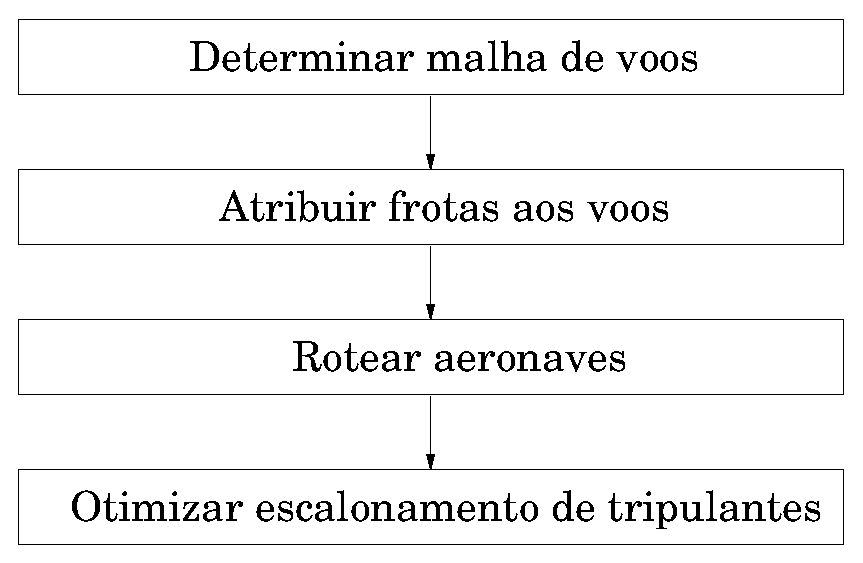
\includegraphics[scale=0.5]{fig/planejamento.eps}
		\caption{Sequência de problemas resolvidos no planejamento de operações de uma empresa
		aérea.}
		\label{fig:planejamento}
	\end{center}
\end{figure}

De forma geral, escalonamento de tripulantes pode ser definido como o problema de se atribuir um
grupo de trabalhadores (uma tripulação) para realizar um conjunto de atividades. No contexto da
aviação, cada tripulante (comandante, co-piloto, comissário, etc) deve ser designado para realizar
um determinado voo da empresa. Tal designação deve ser feita respeitando-se uma série de restrições
impostas pelas agências reguladoras da aviação, bem como regras de regulamentação trabalhista,
restrições operacionais impostas pela própria empresa e acordos trabalhistas entre empregado e
empregador. Dado o grande número de variáveis e restrições envolvidas, assim como a possibilidade de
grandes ganhos econômicos, o problema torna-se bastante interessante, tanto do ponto de vista da
indústria, quanto acadêmico.

Normalmente o problema do escalonamento de tripulantes é dividido em dois subproblemas que são
resolvidos de forma independente e sequencial. O primeiro deles é conhecido como \emph{problema da
determinação de viagens} (PDV), que consiste na obtenção de um subconjunto de viagens, obedecendo as
regras de trabalho impostas pela legislação, com custo mínimo, cobrindo todas os segmentos de voo
exatamente uma vez. Obtida a solução das viagens, um segundo problema é resolvido, conhecido como
\emph{problema da determinação de escalas} (PDE), cujo objetivo é construir as escalas dos
tripulantes, distribuindo as viagens de tal forma que cada viagem seja atribuída exatamente uma vez
para cada tripulante requerido. Na atribuição, visa-se minimizar os custos e garantir distribuição
uniforme de trabalho. A atribuição das viagens também está sujeita a uma série restrições
reguladoras.

Tanto o PDV quanto o PDE têm sido extensamente estudados na literatura~\cite{gopalakrishnan05}. Em
especial, o primeiro deles recebeu mais atenção, principalmente no contexto norte-americano, dada o
seu potencial em produzir economia significativa de custos. No problema da determinação de escalas,
além de minimizar custos, é importante também levar em conta aspectos da qualidade de vida dos
tripulantes. Uma visão geral e esquemática dos dois problemas é apresentada na
Figura~\ref{fig:escalonamento}.

As modelagens matemáticas usuais do PDV e do PDE são semelhantes e baseiam-se em um problema de 
otimização combinatória conhecido por \emph{set partition}. A técnica de resolução comum utilizada 
pode ser descrita como ``gerar-e-otimizar''. Outras abordagens vem sendo recentemente propostas, 
buscando por soluções através de métodos meta-heurísticos. Nos próximos capítulos apresentaremos 
mais detalhes sobre as duas abordagens.

\begin{figure}[htbp]
	\begin{center}
		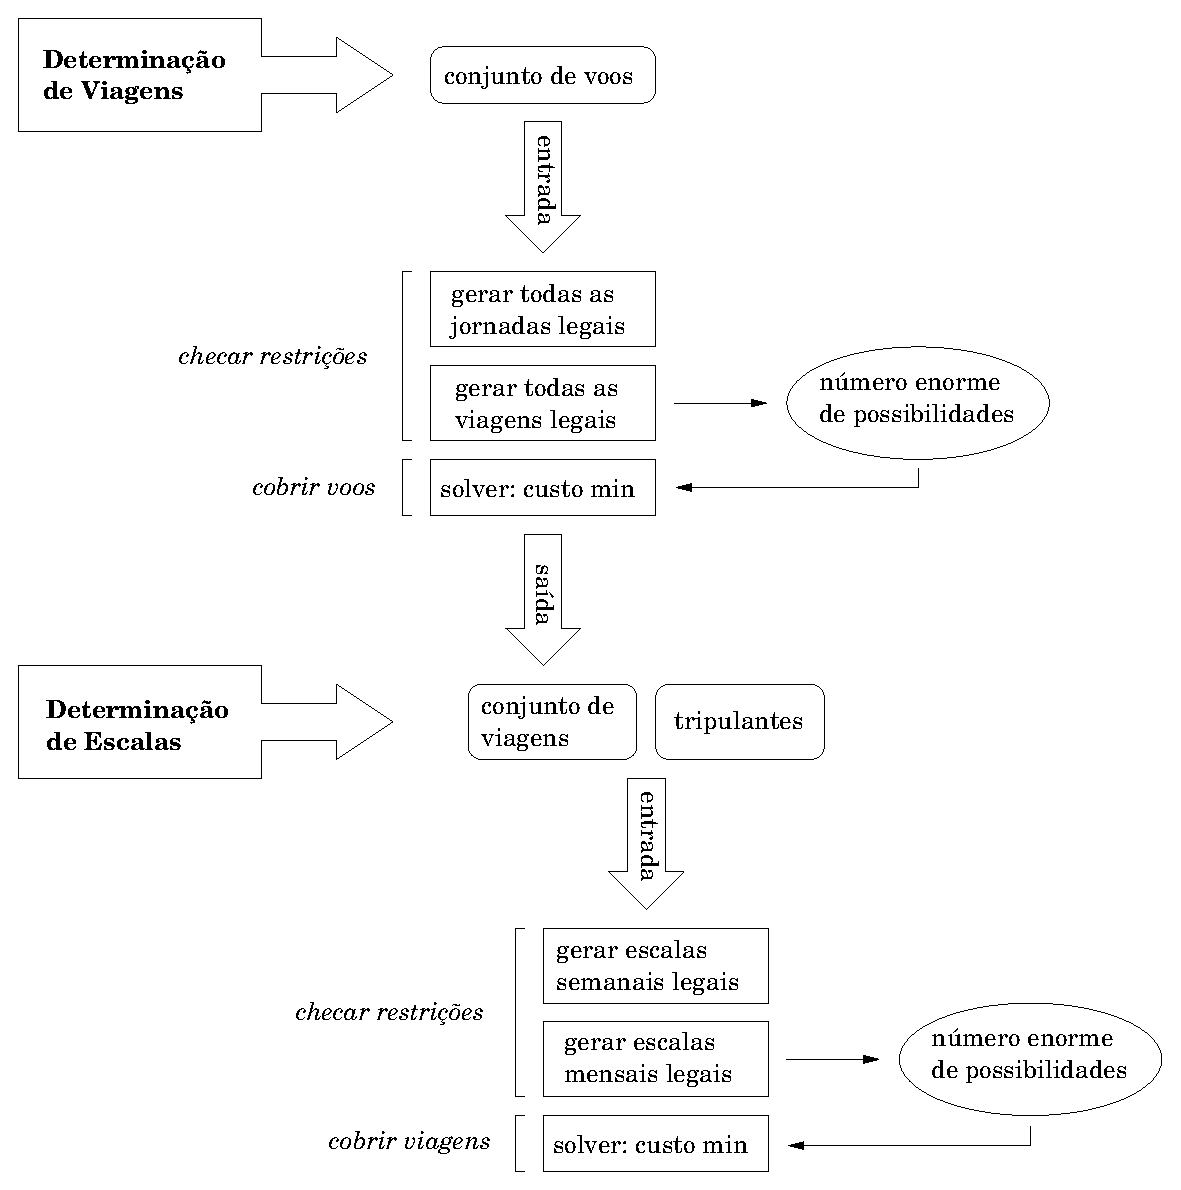
\includegraphics[scale=0.5]{fig/escalonamento.eps}
		\caption{Subproblemas enfrentados na solução do problema de escalonamento de tripulantes 
		(adaptado de~\cite{souai09}).}
		\label{fig:escalonamento}
	\end{center}
\end{figure}

%%%%%%%%%%%%%%%%%%%%%%%%%%%%%%%%%%%%%%%%%%%%%%%%%%%%%%%%%%%%%%%%%%%%%%%%%%%%%%%%%%%%%%%%%%%%%%%%%%%%

\section{Definições}
\label{sec:definicoes}

Antes que possamos apresentar e explorar a estrutura do problema com mais detalhes, faz-se
necessário a introdução de algumas definições e nomenclaturas normalmente utilizadas, as quais serão
amplamente utilizadas neste trabalho.

\begin{itemize}
	\item {\bf Etapa:} é um voo único sem paradas, também chamado de {\bf perna}, {\bf trecho} ou 
	{\bf segmento de voo}.
	\item {\bf Jornada:} conjunto de uma ou mais etapas sequenciais, também chamado de {\bf jornada 
	de trabalho}. 
	\item {\bf Tempo Mínimo de Conexão:} menor intervalo possível de tempo entre duas etapas 
	consecutivas em uma jornada.
	\item {\bf Tempo Máximo de Conexão:} maior intervalo possível de tempo entre duas etapas 
	consecutivos em uma jornada.
	\item {\bf Tempo de Briefing:} tempo mínimo que antecede o início da primeira etapa de uma
	jornada, necessário para o {\it briefing} da tripulação.
	\item {\bf Tempo de Debriefing:} tempo mínimo que sucede o término da último etapa de uma
	jornada,
	necessário para o {\it debriefing} da tripulação.
	\item {\bf Início da Jornada:} horário em que a tripulação deve se apresentar para o início de
	uma jornada. Corresponde ao horário da decolagem da primeira etapa menos o tempo de 
	{\it briefing}. 
	Também chamado de {\bf checkin}.
	\item {\bf Término da Jornada:} horário em que a tripulação encerra suas atividade em uma 
	jornada. Corresponde ao horário de pouso da última etapa mais o tempo de {\it debriefing}.
	Também chamado de {\bf checkout}.
	\item {\bf Base Contratual:} cidade onde uma dado tripulante está domiciliado, também chamada 
	simplesmente de {\bf base}.
	\item {\bf Viagem:} conjunto de jornadas de trabalho, com a primeiro etapa da primeira jornada e
	a última etapa da última jornada começando e terminando na mesma base contratual. 
	Uma viagem também é chamada de {\bf pairing}, ou {\bf rotação}.
	\item {\bf Descanso:} intervalo mínimo de tempo ininterrupto de repouso após uma jornada.
	\item {\bf Pernoite:} intervalo de tempo separando duas jornadas consecutivas de uma viagem.
\end{itemize}

A Figura~\ref{fig:viagem} apresenta o exemplo de uma viagem que ilustra alguns dos conceitos
expostos acima. As etapas na figura estão representadas pelos retângulos mais internos. São
indicados os aeroportos de origem e destino, bem como os horários de decolagem e pouso. As
jornadas são indicadas pelos retângulos pontilhados, englobando uma cadeia de etapas. A base 
contratual considerada é CGH (São Paulo). 

\begin{figure}[htbp]
	\begin{center}
		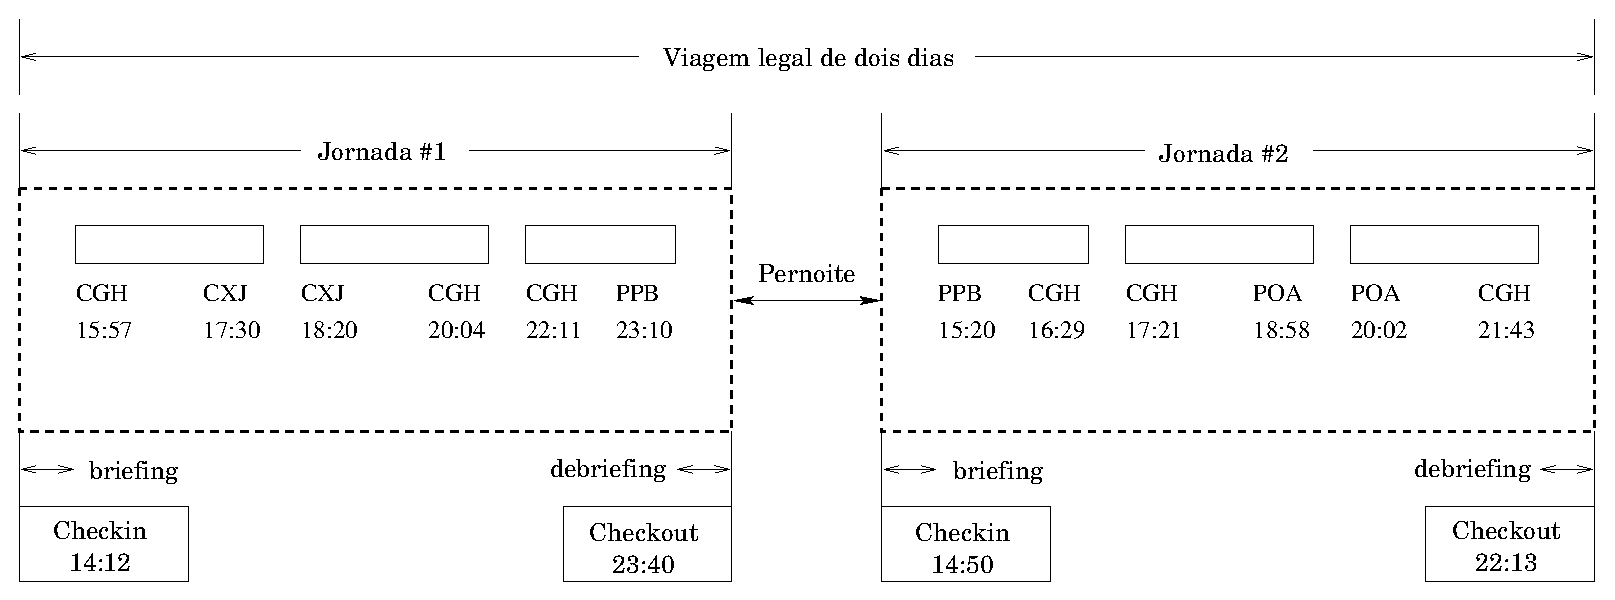
\includegraphics[scale=0.5]{fig/viagem.eps}
		\caption{Exemplo de uma viagem de dois dias para a base CGH.}
		\label{fig:viagem}
	\end{center}
\end{figure}

%%%%%%%%%%%%%%%%%%%%%%%%%%%%%%%%%%%%%%%%%%%%%%%%%%%%%%%%%%%%%%%%%%%%%%%%%%%%%%%%%%%%%%%%%%%%%%%%%%%%

\section{Formulação do PDV}
\label{sec:formulacao}

No problema da determinação das viagens, tem-se como entrada o conjunto de voos a ser operado pela
empresa, o conjunto de bases contratuais dos tripulantes, as regras de trabalho que ditam a
construção de viagens legais e uma estrutura de custo (mais detalhes na 
Seção~\ref{sec:regras_e_custos}). A saída, então, deve ser um conjunto de viagens que cubra todos os
voos operados exatamente e uma vez e que tenha o custo mínimo (veja Figura~\ref{fig:pdv}).

\begin{figure}[htbp]
	\begin{center}
		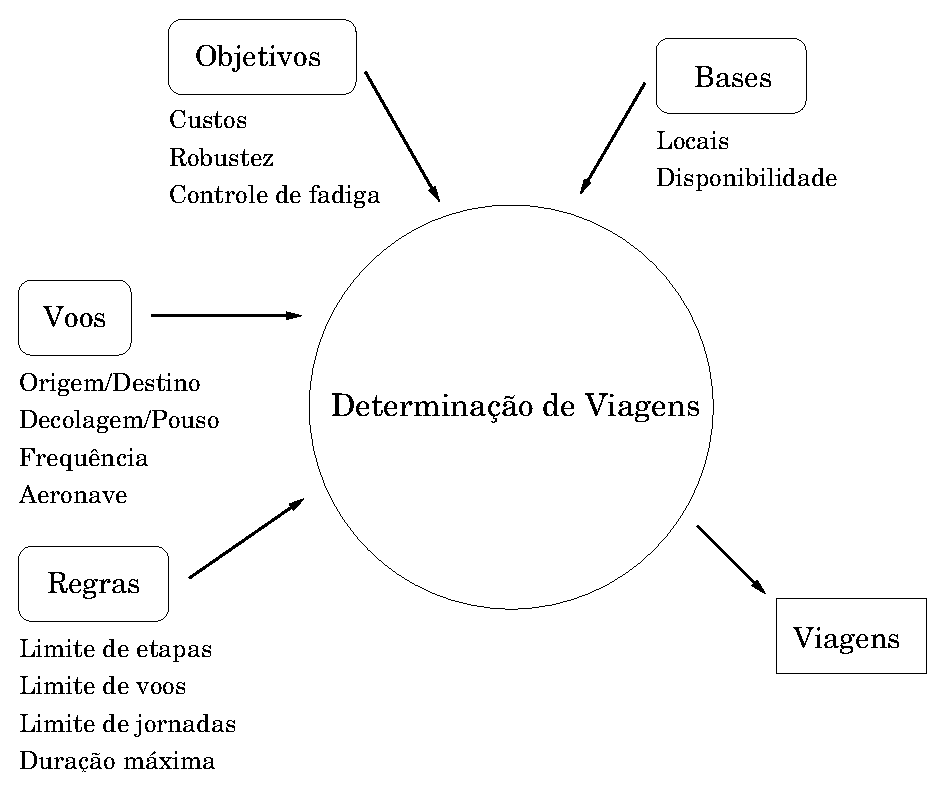
\includegraphics[scale=0.5]{fig/pdv.eps}
		\caption{Representação do problema da determinação de viagens (PDV).}
		\label{fig:pdv}
	\end{center}
\end{figure}

Normalmente os voos das companhias aéreas apresentam uma frequência regular de oferecimento, sendo
que a maioria deles operam diariamente. Outros são oferecidos apenas em alguns dias fixos da semana
e poucos são oferecidos vez ou outra no mês. Costuma-se então inicialmente resolver o problema
diário, onde se assume que todos os voos são repetidos diariamente. Note que para o problema diário,
viagens de vários dias com etapas repetidas são inviáveis. Um segmento de voo repetido causaria o
efeito de mais de uma tripulação ser atribuída para realização dessa etapa, uma vez que quando se
faz a implementação da solução diária, uma tripulação distinta é atribuída a cada um dos dias da
viagem.

O problema semanal é mais complicado porque envolve um maior número de etapas consideradas. De
qualquer forma, a solução do problema semanal pode ser obtido a partir de um ajuste da solução do
problema diário, sem perda significativa de custo~\cite{gopalakrishnan05}. A solução do problema
mensal completo segue da solução do problema semanal. Como a maior parte da redução de custos está
associada à resolução do problema diário, ele se torna o mais importante. Daqui em diante trataremos
apenas do problema diário.

Uma outra simplificação do problema está no fato que os tripulantes são habilitados para operar
apenas um tipo, ou família, de aeronaves dentro de uma frota. Assim, fatora-se o problema da
determinação das viagens por tipo de aeronave. Para cada tipo, resolve-se um PDV considerando apenas
as etapas operadas por aquele tipo. As viagens assim geradas são atribuídas aos tripulantes
habilitados no tipo ao se resolver o PDE.

Há uma formulação natural para o PDV em termos de um problema de programação linear. Suponha que
seja possível gerar e enumerar todas as $n$ viagens associadas a uma dada entrada do problema
contendo $m$ etapas a serem cobertas. Seja $x_j \in \{0, 1\}$ uma variável de decisão que assume o
valor 1 se a viagem $j$ for escolhida na solução de custo mínimo e 0 caso contrário. Então, o PDV
pode ser modelado da seguinte forma:
%
\begin{eqnarray} \label{eq:sppv}
	\text{minimizar} && \displaystyle \sum_{j=1}^n c_j x_j \nonumber \\
	\text{sujeito à} && \displaystyle \sum_{j=1}^n a_{ij} x_j = 1 \ev \;\; i = 1, \ldots, m \\
		               && x_j \in \{0, 1\} \ev \;\; j = 1, \ldots, n \ep \nonumber
\end{eqnarray} 
%
Os coeficientes $a_{ij}$ são definidos por (matriz de incidência)
%
\begin{equation*}
	a_{ij} = \left\{
	\begin{array}{ll}
			1 \ev & \text{se a viagem $j$ cobre a etapa $i$} \\
			0 \ev & \text{caso contrário}
	\end{array}
	\right.
\end{equation*}

As restrições em (\ref{eq:sppv}) garantem que cada etapa seja coberta exatamente uma vez por alguma
viagem. Existe ainda uma formulação alternativa onde as restrições são dadas por
%
\begin{equation} \label{eq:dh} 
	\sum_{j=1}^n a_{ij} x_j \geq 1 \, , \;\; i = 1, \ldots, m \ep
\end{equation} 
%
Nesse caso uma mesma etapa pode ser coberta por mais de uma viagem e o problema se torna um
\emph{set cover}. Do ponto de vista do escalonamento, se uma etapa é coberta por mais
de uma viagem, então uma tripulação estará trabalhando nessa etapa e as demais viajando de
passageiro (situação conhecida por \emph{deadheading}). As vezes essa situação é necessária para
que se garanta viabilidade da solução. Se o preço a se pagar pela operação com \emph{deadheading} 
for essencialmente o mesmo de uma operação normal, então não há alteração significativa no custo 
da viagem associada. Isso permite que o problema seja modelado com as restrições (\ref{eq:dh}) 
sem alterar a estrutura de custos.

É comum a inserção de restrições adicionais ao modelo que garantem uma distribuição de trabalho
entre as bases compatível com os recursos disponíveis em cada base. Se o número total de bases do
problema considerado é $r$, então as \emph{restrições de bases} são expressas por
%
\begin{equation} \label{eq:bases}
	H_k^L \leq \sum_{j=1}^n h_{kj} x_j \leq H_k^U \, , \;\; k = 1, \ldots, r \ev
\end{equation}
%
onde $H_k^L$ é o número mínimo de horas disponíveis na base $k$ e $H_k^U$ é seu número máximo. 
Note que $H_k^L$ pode ser diferente de zero desde que se exija que não mais do que um certo número 
de tripulantes fiquem de reserva. O coeficiente $h_{kj}$ dá o número de horas necessárias para 
efetuar a viagem $j$ ($h_{kj} = 0$ se a viagem $j$ não pertencer à base $k$).

O grande problema com a formulação (\ref{eq:sppv}) está no enorme número de variáveis geradas, mesmo
nos casos das instâncias pequenas (poucas etapas diárias). A Tabela~\ref{tab:viagens} ilustra o
número de viagens legais geradas, com duração máxima de 3 ou 4 dias, para diversas frotas de
aeronaves. O número enorme de variáveis está associada com a natureza combinatória do problema. A
maioria das empresas aéreas operam em aeroportos conhecidos como \emph{hubs}, onde um grande número
de aeronaves chegam e partem em um mesmo intervalo de tempo, possibilitando que os passageiros
efetuem suas conexões para uma variedade de destinos em pouco tempo. Esse tipo de estrutura em rede 
leva à explosão no número de viagens legais que podem ser construídas~\cite{graves93}. Note da
Tabela~\ref{tab:viagens} que apesar do número de viagens ser gigantesco, o número de 
jornadas tem um valor mais gerenciável.

\begin{table}[ht]
	\begin{center}
		\begin{tabular}{|c||c|c|c|c|c|}
			\hline
			{\bf Frota} & {\bf Max Dias} & {\bf Etapas} & {\bf Bases} & {\bf Jornadas} & 
			{\bf Viagens} ($\times 10^6$) \\
			\hline
			AAS80 & 3 & 1.152 & 12 & 690.000 & 48.400 \\
			\hline
			AA757 & 3 & 251 & 15 & 7.000 & 1 \\
			\hline
			AA727 & 3 & 375 & 11 & 31.000 & 36 \\
			\hline
			AAF10 & 4 & 307 & 3 & 55.000 & 63.200 \\
			\hline 
			UA737 & 4 & 773 & 7 & 568.000 & 100.000.000 \\
			\hline
			USDC9 & 4 & 478 & 4 & 562.000 & 105.000.000 \\
			\hline
		\end{tabular}
		\caption{Jornadas e viagens legais geradas para um conjunto de frotas de aeronaves de companhias
		norte-americanas (fonte:~\cite{anbil98}).}
		\label{tab:viagens}
	\end{center}
\end{table}

Como o problema de partição é NP-difícil~\cite{garey79}, a aplicação de métodos diretos de
otimização é impraticável para qualquer situação real. Discutiremos esse ponto na
Seção~\ref{sec:preliminar}. Os métodos de solução normalmente envolvem algum tipo de heurística e/ou
algum critério de parada que leva a soluções sub-ótimas.

%%%%%%%%%%%%%%%%%%%%%%%%%%%%%%%%%%%%%%%%%%%%%%%%%%%%%%%%%%%%%%%%%%%%%%%%%%%%%%%%%%%%%%%%%%%%%%%%%%%%

\section{Objetivos e Estrutura}
\label{sec:objetivos}

Neste trabalho focamos no problema da determinação das viagens. Os objetivos foram estudar a 
literatura, entender e implementar alguns dos métodos de solução disponíveis, aplicando-os
no contexto de companhias aéreas brasileiras e, por fim, analisar os resultados obtidos.

O contexto brasileiro difere significativamente dos contextos estrangeiros no que se refere à 
estrutura de custos e regras que ditam a viabilidade de uma viagem. Como os trabalhos estudados na
literatura se referem ao escopo norte-americano e europeu, tivemos por objetivo também efetuar as 
devidas adaptações na tentativa de solucionar problemas de companhias aéreas brasileiras.

Esta monografia está estruturada da seguinte forma: neste capítulo faz-se uma introdução e
contextualização do problema em estudo. Em seguida, no Capítulo~\ref{cap:geracao} apresentamos o
método de geração de viagens, com destaque especial na estrutura de custos e regras de viabilidade.
Um exemplo explícito é apresentado. No Capítulo~\ref{cap:heuristicas} apresentamos as tês
heurísticas implementadas neste trabalho, a saber, um método de busca local, um algoritmo genético
híbrido e um procedimento de geração de colunas. O Capítulo~\ref{cap:resultados} mostra os
resultados obtidos aplicando-se as heurísticas estudadas a algumas instâncias reais do problema. Em
particular, mostramos a redução do custo da solução em função do número de iterações que controla a
evolução dos algoritmos. Finalmente, no Capítulo~\ref{cap:conclusao} destacamos algumas conclusões e
comparações de resultados. Listamos também alguns pontos de melhorias, dificuldades com o projeto e
perspectivas futuras. 

A segunda parte desta monografia apresenta o conteúdo subjetivo, destacando a opinião e as
impressões de cada autor sobre o curso do BCC/IME e a relação com este projeto
(Capítulo~\ref{cap:sub}).

\zerar
\chapter{Geração de Viagens}
\label{cap:geracao}

Todos os métodos de solução do PDV (exatos ou heurísticos) exigem um mecanismo de geração 
explícita de viagens válidas, as quais representam as variáveis que desejamos otimizar. 

A geração pode ser eficientemente implementada através de uma busca em uma rede de voos. 
O resultado da busca depende explicitamente das regras de trabalho impostas pelo contexto do
problema. As viagens geradas apresentam um custo também intimamente ligado ao contexto e ao 
objetivo que se deseja atingir. 

Neste capítulo apresentaremos mais detalhes sobre o procedimento de geração de viagens. Ao final,
será exibido um exemplo explícito.

%%%%%%%%%%%%%%%%%%%%%%%%%%%%%%%%%%%%%%%%%%%%%%%%%%%%%%%%%%%%%%%%%%%%%%%%%%%%%%%%%%%%%%%%%%%%%%%%%%%%

\section{Regras de Trabalho e Estrutura de Custo}
\label{sec:regras_e_custos}

É importante explicitar os tipos de restrições e a estrutura de custo envolvidos no problema, em 
especial no contexto brasileiro, já que há uma diferença significativa com relação aos contextos 
norte-americano e europeu, normalmente analisados na literatura.

No caso do PDV, a geração de uma viagem é regida por uma série de regras impostas pela Agência
Nacional de Aviação Civil (ANAC), além de restrições impostas por leis trabalhistas e acordos
contratuais. Uma viagem é dita válida (ou legal) se ela obedecer todas as regras impostas pela
legislação em questão. Abaixo, apresentamos os valores típicos das regras que regem a construção de
uma viagem em uma empresa de aviação ergular do Brasil, com voos de curto e médio alcance (veja a
Seção~\ref{sec:definicoes} para as defininições):

\begin{itemize}
	\item Duração máxima de uma jornada de trabalho: 11 horas;
	\item Número máximo de horas de voo em uma jornada: 9 horas e 30 minutos;
	\item Número máximo de pousos em uma jornada: 6 pousos;
	\item Descanso mínimo entre jornadas: 12 horas;
	\item Tamanho máximo de uma viagem: 6 dias;
	\item Tempo mínimo de conexão: 30 minutos;
	\item Tempo máximo de conexão: 4 horas;
	\item Número máximo de trocas de aeronave em uma jornada: 2 trocas;
	\item Tempo de {\it briefing}: 30 minutos fora de base e 45 minutos na base;
	\item Tempo de {\it debriefing}: 30 minutos.
\end{itemize}

O custo de uma viagem está associado à produtividade mais os custos referentes à estadia do 
tripulante quando este precisar pernoitar fora da base, além das diárias de alimentação. Uma 
expressão típica para calcular o custo $c_p$ de uma viagem $p$ é dada por
%
\begin{equation} \label{eq:custov} 
	c_p = \sum_{d \in D_p} c_d \, , \;\;
	c_d = \alpha_0 \left[t_d - \left(tp_d - \sum_{i \in I_d} t_i\right)\right] + cp_d \ev
\end{equation} 
%
onde
%
\begin{itemize}
	\item[$D_p$:] conjunto de jornadas que constituem a viagem $p$;
	\item[$c_d$:] custo da jornada $d$;
	\item[$\alpha_0$:] custo da hora de trabalho do tripulante;
	\item[$t_d$:] duração da jornada $d$ (em horas);	
	\item[$tp_d$:] tempo de preparação ({\it briefing} mais {\it debriefing}) usado na jornada $d$;
	\item[$I_d$:] conjunto de etapas que compõe a jornada $d$;
	\item[$t_i$:] duração da etapa $i$, incluindo o tempo mínimo de conexão;
	\item[$cp_d$:] custo do pernoite mais diárias de alimentação da jornada $d$.
\end{itemize}
%
Note que a expressão que multiplica $\alpha_0$ em (\ref{eq:custov}) representa o tempo que o
tripulante passou trabalhando sem estar voando, portanto representa uma medida de produtividade.
Quanto mais cara a viagem, menor é a produtividade do tripulante.

A estrutura descrita acima refere-se a um modelo padrão para companhias aéreas brasileiras.
Fora do Brasil, entretanto, a estrutura do custos pode ser diferente. Nos Estados Unidos, por 
exemplo, o custo de uma viagem é dado por uma função não-linear de diferentes custos. 
Especificamente, o custo de uma viagem $p$ é dado por
%
\begin{equation*}
	c_p = \max\left\{\sum_{d \in D_p} MIN\_GRT_d \ev \sum_{d \in D_p} FLY\_TIME_d \ev 
	TIME\_AWAY_p \right\} \ev
\end{equation*}
%
onde $MIN\_GRT_d$ é o mínimo de garantia oferecido ao tripulante ao voar a jornada $d$, 
$FLY\_TIME_d$ é o tempo de voo da jornada $d$ (pode ser multiplicado por algum fator) e
$TIME\_AWAY_p$ é o tempo total que o tripulante passa fora de sua base na viagem $p$ (também pode
ser multiplicado por algum fator). Observe assim que, nesse modelo, o custo de cada etapa depende da
viagem em que ela está incluída.

%%%%%%%%%%%%%%%%%%%%%%%%%%%%%%%%%%%%%%%%%%%%%%%%%%%%%%%%%%%%%%%%%%%%%%%%%%%%%%%%%%%%%%%%%%%%%%%%%%%%

\section{Gerador de Viagens}
\label{sec:gerador_viagens}

O primeiro passo em direção à solução do PDV consiste na implementação de um gerador de viagens 
eficiente que seja capaz de produzir um grande número de viagens válidas em pouco tempo. Como já
mencionamos, os métodos de resolução de (\ref{eq:sppv}) baseiam-se no conceito de 
``gerar-e-otimizar'', e já que as rotinas de otimização estão normalmente prontas em pacotes 
fechados, a parte de geração é de grande importância.

Uma viagem pode ser vista como um caminho especial em um grafo estruturado. Esse grafo é chamado de
\emph{rede de voos} e será detalhado a seguir. 

As etapas na rede de voos podem ser representadas como nós ou arcos. Escolhemos a representação em
termos de arcos. Os nós da rede representam as saídas e chegadas de cada etapa, bem como uma fonte
$s$ e um sorvedouro $t$. Existe um arco representando cada etapa da malha de voos. Para o problema
diário, replicamos cada arco quantas vezes for o número máximo de dias permitido em um viagem. O
conjunto de arcos será denotado por $\calA$.

O nó fonte é ligado ao nó de saída de cada etapa que origina-se em uma base específica. O nó de
chegada de cada etapa que termina nessa base é ligado ao sorvedouro. Existem ainda arcos
representando conexões válidas entre etapas. Um par de etapas terá um arco de conexão entre elas se
o aeroporto de chegada do primeiro corresponder ao aeroporto de saída do segundo e se o intervalo de
tempo entre a chegada e a saída estiver dentro dos limites necessários para se estabelecer uma
conexão válida em uma jornada ou descanso regular entre jornadas. 

É fácil notar que toda viagem válida é representada por um caminho $s-t$ na rede de voos. Porém,
existem caminhos $s-t$ que não representam viagens válidas pois podem desrespeitar alguma regra de
trabalho, embora as conexões possíveis sejam válidas. A estrutura da rede garante que não seja feita
nenhuma conexão entre duas etapas que não tenham seus respectivos destino e origem coincidentes no
espaço e no tempo. Entretanto, não garante, por exemplo, que o número máximo de horas de voo
permitido em uma jornada seja excedido. 

O gerador de viagens funciona aplicando um algoritmo de busca em profundidade à rede de voos. O
algoritmo inicia-se no nó de origem $s$ e explora todas a conexões viáveis $(i, j) \in \calA$, até
retroceder. O processo de busca em profundidade controla a viabilidade das viagens, levando em conta
a duração máxima das jornadas, limites de horas de voo e de pousos, etc (ou seja, verifica as regras
de trabalho ao atravessar cada arco).

%%%%%%%%%%%%%%%%%%%%%%%%%%%%%%%%%%%%%%%%%%%%%%%%%%%%%%%%%%%%%%%%%%%%%%%%%%%%%%%%%%%%%%%%%%%%%%%%%%%%

\section{Exemplo}
\label{sec:exemplo}

A tabela abaixo mostra um conjunto fictício (para fins de ilustração) de 7 etapas operadas 
diariamente entre as localidades A, B, C e D. O exemplo é adaptado de~\cite{barnhart03}. 

\begin{table}[ht]
	\begin{center}
		\begin{tabular}{ccccc}
			{\bf \# Etapa} & {\bf Origem} & {\bf Destino} & {\bf Saída} & {\bf Chegada} \\ \hline
			1 & A & B & 08:00 & 09:00 \\
			2 & B & C & 10:00 & 11:00 \\
			3 & C & D & 13:00 & 14:00 \\
			4 & C & A & 15:00 & 16:00 \\
			5 & D & A & 15:00 & 16:00 \\
			6 & A & B & 17:00 & 18:00 \\
			7 & B & C & 11:00 & 12:00 \\
		\end{tabular}
	\end{center}
\end{table}

A rede de voos (parcial) para uma base contratual A é ilustrada na Figura~\ref{fig:rede}, onde são
apresentadas algumas das conexões válidas possíveis para clareza do desenho. O caminho vermelho
na figura representa uma viagem válida com dois dias de duração. 

A partir da rede apresentada, montamos as seguintes jornadas válidas (os números representam os
números das etapas)
%
\begin{eqnarray*}
	&& D_1 = \{1\} \ev \hsp D_2 = \{2\} \ev \hsp D_3 = \{3\} \ev \hsp D_4 = \{4\} \\
	&& D_5 = \{5\} \ev \hsp D_6 = \{6\} \ev \hsp D_7 = \{7\} \ev \hsp D_8 = \{1, 2\} \\
	&& D_9 = \{1, 7 ,3\} \ev \hsp D_{10} = \{2, 3\} \ep 
\end{eqnarray*}

Assumindo que as localidades A, B e D sejam bases contratuais, geramos seis viagens, que podem ser
expressas em termos das jornadas como 
%
\begin{eqnarray*}
	&& P_1 = \{D_4, D_8\} \ev \hsp P_2 = \{D_9, D_5\} \ev \hsp P_3 = \{D_5, D_6, D_{10}\} \\
	&& P_4 = \{D_4, D_6, D_7\} \ev \hsp P_5 = \{D_1, D_7, D_4\} \ev \hsp P_6 = \{D_7, D_4, D_9\}
\ep 
\end{eqnarray*}

Note que a viagem $P_6$ cobre a etapa $7$ duas vezes, então ela não é válida e deve ser 
desconsiderada. Supondo que os custos associados às viagens sejam $c_1 = c_2 = c_3 = c_4 = 4$ e
$c_5 = 5$, a partir de (\ref{eq:sppv}) obtemos o seguinte problema ($x_i \in \{0, 1\}$, 
$i=1, \ldots, 5$):
%
\begin{equation*}
	\begin{array}{lllllllllllll}
		\text{min} & 4x_1 & + & 4x_2 & + & 4x_3 & + & 4x_4 & + & 5 x_5 & & & \vsp \\ 
		& x_1 & + & x_2 & & & & & + & x_5 & = & 1 & \text{(etapa 1)} \vsp \\
		& x_1 & & & + & x_3 & & & & & = & 1 & \text{(etapa 2)} \vsp \\
		& & & x_2 & + & x_3 & & & & & = & 1 & \text{(etapa 3)} \vsp \\
		& x_1 & & & & & + & x_4 & + & x_5 & = & 1 & \text{(etapa 4)} \vsp \\
		& & & x_2 & + & x_3 & & & & & = & 1 & \text{(etapa 5)} \vsp \\
		& & & & & x_3 & + & x_4 & & & = & 1 & \text{(etapa 6)} \vsp \\
		& & & x_2 & & & + & x_4 & + & x_5 & = & 1 & \text{(etapa 7)}
	\end{array}
\end{equation*}

Se pelo menos 3 horas e no máximo 6 horas estejam disponíveis nas bases A e D, e no máximo 5 horas 
na base C, então as restrições de bases (\ref{eq:bases}) são
%
\begin{equation*}
	\begin{array}{ll}
		3 \leq 4 x_2 + 3 x_5 \leq 6 & \text{(base A)} \vsp \\
		0 \leq 3 x_1 + 3 x_4 \leq 5 & \text{(base C)} \vsp \\
		3 \leq 4 x_3 \leq 6 & \text{(base D)}
	\end{array}
\end{equation*}

A solução ótima para o problema formulado usa as viagens 3 e 5 ($x_3 = x_5 = 1$, 
$x_1 = x_2 = x_4 =  0$) e tem um custo total igual à 9. Por se tratar de um problema pequeno, a
resolução do mesmo pode ser obtida por qualquer pacote de otimização linear.

\begin{figure}[htbp]
	\begin{center}
		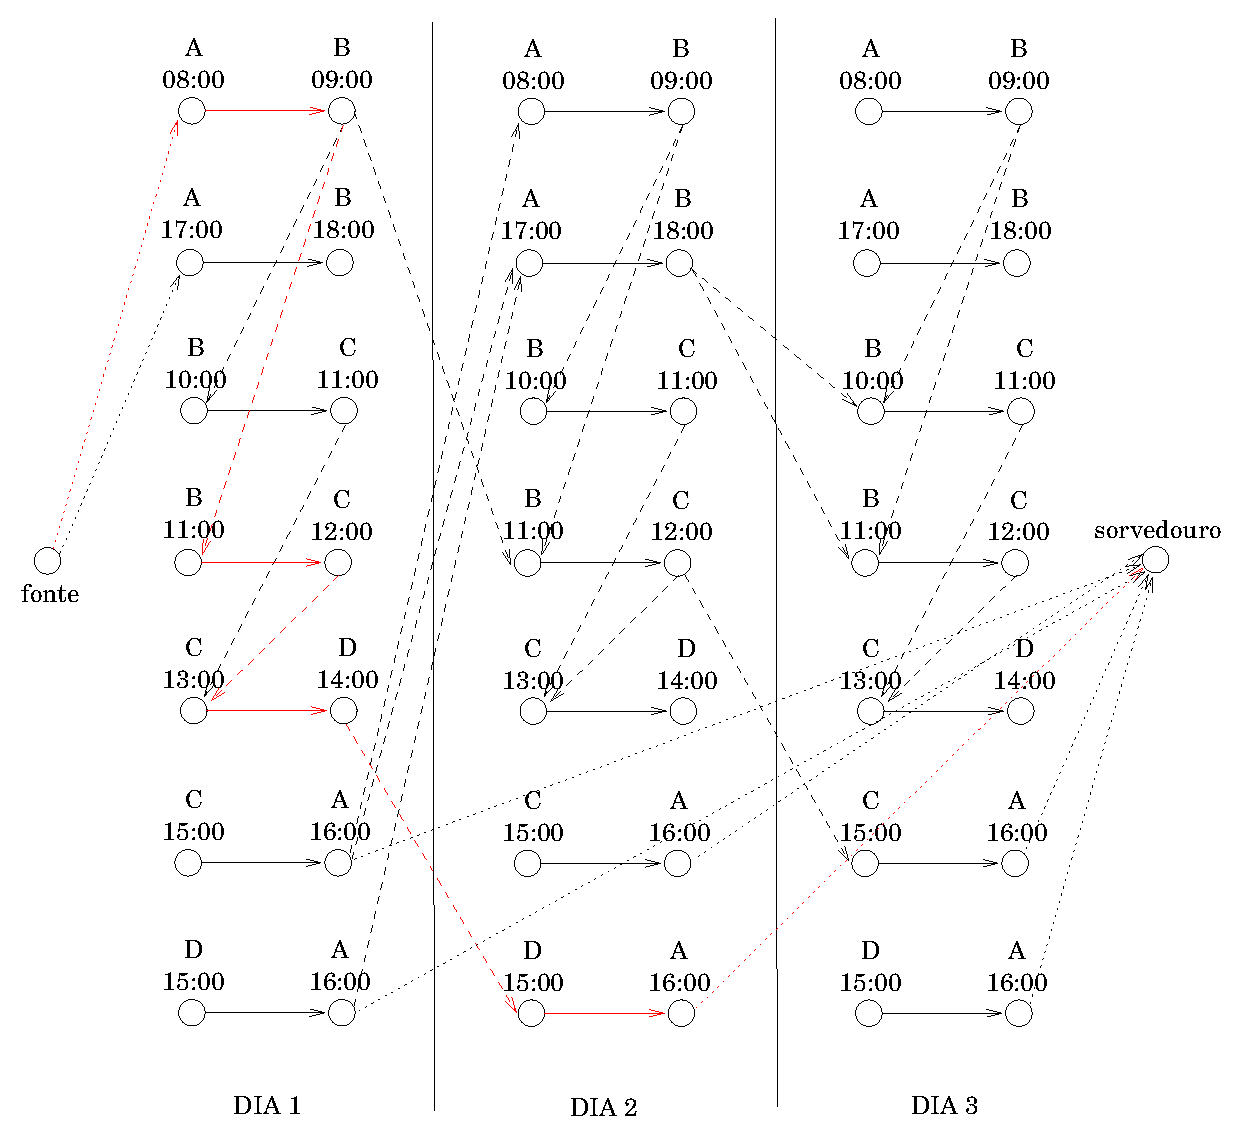
\includegraphics[scale=0.80]{fig/rede.eps}
		\caption{Rede de voos referente às 7 etapas do exemplo ilustrativo. Considerou-se
		viagens de no máximo 3 dias, por isso os nós são replicados três vezes para o
		problema diário. A base dos tripulantes considerada foi a localidade A, dando origem
		às ligações da fonte e do sorvedouro.
		Arcos tracejados representam conexões válidas entre localidades. O caminho em
		vermelho representa uma das viagens possíveis.}
		\label{fig:rede}
	\end{center}
\end{figure}

%%%%%%%%%%%%%%%%%%%%%%%%%%%%%%%%%%%%%%%%%%%%%%%%%%%%%%%%%%%%%%%%%%%%%%%%%%%%%%%%%%%%%%%%%%%%%%%%%%%%


\zerar
\chapter{Heurísticas}
\label{cap:heuristicas}

Os métodos exatos de solução do PDV resolvem, utilizando técnicas de otimização, o modelo de
programação linear inteiro (\ref{eq:sppv}). Dessa forma, uma solução ótima global para o problema é
obtida~\cite{anbil91b}. A resolução pelo otimizador é feita inicialmente considerando uma versão
relaxada do problema, \ie, permitindo que as variáveis $x_j$ assumam valores {\it reais} entre 0 e
1. A seguir, o problema relaxado é resolvido pelo método Simplex, ou alguma especialização do mesmo,
o que gera uma solução ótima fracionária $x^\ast$. A partir de $x^\ast$, empregando-se um esquema
{\it branch-and-bound}, ou {\it branch-and-cut}, obtém-se a melhor solução inteira. Vale ressaltar
que tais procedimentos de enumeração implícita consomem tempo e memória exponencial no número de
variáveis. Assim, a aplicação de tais métodos limita-se a instâncias pequenas.

Diversos métodos heurísticos foram desenvolvidos ao longo dos anos para lidar com o número
gigantesco de variáveis do problema e a incapacidade dos otimizadores lidarem com elas. Uma
listagem descritiva das principais heurísticas pode ser encontrado em~\cite{gopalakrishnan05}.

Após análise da literatura, resolvemos estudar mais a fundo e implementar três alternativas: um
método de busca local, um algoritmo genético híbrido e um procedimento de geração de colunas. 

Busca local foi a primeira heurística historicamente adotada pelas empresas para resolver seus
grandes problemas de escalonamento, levando a resultados satisfatórias~\cite{gershkoff89} na década
de 80. Dentre as meta-heurísticas, algoritmos genéticos vem sendo mais recentemente aplicados como
forma de se obter uma solução aproximada~\cite{kornilakis02}. Os resultados para problemas grandes,
entretanto, ainda não são satisfatórios. Finalmente, procedimentos de geração de colunas representam
o estado-da-arte dos métodos de solução, e constituem a base dos poderosos métodos do tipo {\it
branch-and-price}~\cite{vance97}.

%%%%%%%%%%%%%%%%%%%%%%%%%%%%%%%%%%%%%%%%%%%%%%%%%%%%%%%%%%%%%%%%%%%%%%%%%%%%%%%%%%%%%%%%%%%%%%%%%%%%

\section{Refatornado o Modelo}
\label{sec:refatorando}

Antes de explicarmos em mais detalhes cada uma das heurísticas estudadas, vamos fazer uma pequena
modificação ao modelo (\ref{eq:sppv}). Observe que o mesmo não admite a existência de {\it
deadheading}, \ie, tripulação viajando como passageiro. Em algumas situações isso pode implicar na
inviabilidade do problema.

A formulação que adotaremos a seguir modela o problema conhecido por {\it set cover}. Ele é bastante
similar ao {\it set partition}, porém admite a ocorrência de {\it deadheading} na solução final,
tornando possível a existência de soluções viáveis para o problema original.

As restrições no {\it set cover} são dadas pelas equações (\ref{eq:dh}), onde permite-se que 
uma etapa seja coberta mais do que uma vez. Sendo $m$ o número de etapas a serem cobertas, podemos 
adicionar $m$ variáveis artificiais inteiras $y_i$, $i = 1, \ldots, m$, onde $y_i$ representa o 
número de vezes que a etapa $i$ é coberta como {\it deadhead}. Considerando um custo $d_i$ cada vez 
que a etapa $i$ é utilizada como {\it deadhead}, o problema de programação linear resultante é
%
\begin{eqnarray} \label{eq:scpdv}
	\text{minimizar} && \displaystyle \sum_{j=1}^n c_j x_j + \sum_{i=1}^m d_i y_i \nonumber \\
	\text{sujeito à} && \displaystyle \sum_{j=1}^n a_{ij} x_j - y_i = 1 \ev \;\; i = 1, \ldots, m \\
	                 && x_j \in \{0, 1\} \ev \;\; j = 1, \ldots, n \nonumber \\
	                 && y_i \geq 0 \ev \;\; i = 1, \ldots, m \ep \nonumber
\end{eqnarray}

A adoção de custos altos associados às varáveis $y_i$ faz com que elas sejam naturalmente expulsas 
da base no final, levando a uma solução livre de {\it deadheading}, se alguma existir. Isso funciona
mais ou menos como o método-$M$ na primeira fase do algoritmo Simplex para obtenção de uma solução 
viável básica.

A vantagem do modelo (\ref{eq:scpdv}) é que com ele fica mais fácil encontrar uma solução viável
inicial para o problema. Como é permitido a sobreposição de etapas, podemos ir percorrendo a rede
de voos e ir gerando as viagens. Toda vez que uma nova viagem gerada cobrir uma perna não coberta,
armazenamos essa viagem na solução. Paramos quando todas as pernas tiverem sido cobertas.

%%%%%%%%%%%%%%%%%%%%%%%%%%%%%%%%%%%%%%%%%%%%%%%%%%%%%%%%%%%%%%%%%%%%%%%%%%%%%%%%%%%%%%%%%%%%%%%%%%%%

\section{Busca Local}
\label{sec:metodos_busca}

Busca local é uma abordagem geral utilizada para encontrar soluções de boa qualidade para problemas
de otimização combinatória difíceis, em tempo aceitável. O método é baseado em uma exploração 
iterativa de vizinhos da solução tentando melhorar a solução atual através de alterações locais.

A solução encontrada por um algoritmo de busca local tem a garantia apenas de ser ótima com relação
a alterações locais e, em geral, não será a solução ótima global.

O método de busca local no contexto do PDV é bastante simples e foi um dos primeiros a ser utilizado
na tentativa de melhorar uma solução viável do problema (\ref{eq:scpdv}). Basicamente o método
consiste em escolher aleatoriamente um número pequeno, $k$, de viagens da solução viável inicial
(subproblema) e, a partir da lista de etapas cobertas e tripuladas por essas viagens, gerar
explicitamente todas as possíveis viagens legais usando o gerador. Como o número de etapas não é
muito grande, o número de variáveis geradas é gerenciável. O modelo (\ref{eq:scpdv}) é então
resolvido pelo otimizador para todas essas variáveis, obtendo-se um novo conjunto de viagens que
cobre o lista inicial de etapas. Se o custo desse novo conjunto de viagens for menor do que o
original, então as viagens originais serão substituídas na solução inicial. O processo é iterado um
número máximo de vezes (ou um tempo máximo de execução), ou até que não haja variação significativa
do custo (mínimo local), de tal forma que o custo sempre seja reduzido a cada passo.

Um fluxograma da execução do algoritmo é apresentado na Figura~\ref{fig:busca_local}. Note que se
tivermos uma boa rotina de geração de viagens e otimização, o método pode ser facilmente 
implementado. O sucesso na aplicação do método depende crucialmente do fato de sermos capazes de 
resolver eficientemente o PLI (\ref{eq:scpdv}) para um número pequeno de variáveis.

\begin{figure}[htbp]
	\begin{center}
		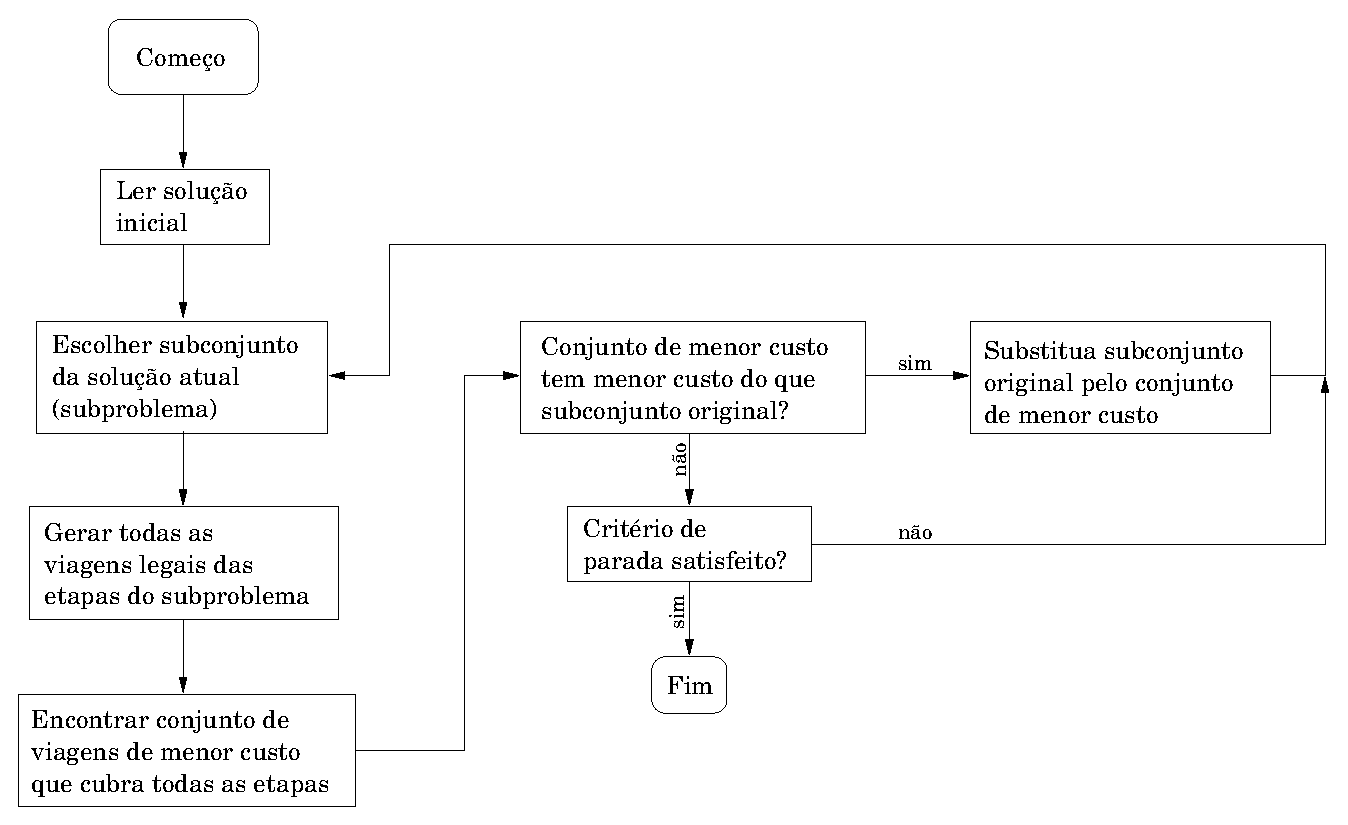
\includegraphics[scale=0.6]{fig/localsearch.eps}
		\caption{Algoritmo para o método da busca local. O fluxograma mostra como o processo de 
		otimização repete o loop de gerar viagens e encontrar um subconjunto ótimo otimizar até que
		algum critério de parada seja atingido.}
		\label{fig:busca_local}
	\end{center}
\end{figure}

A escolha do subproblema de forma aleatória é uma das mais simples possíveis. Algumas outras 
propostas foram consideradas~\cite{anbil91a,arabeyre69}. Entretanto, a escolha aleatória ainda
parece ser a que apresenta melhor custo-benefíficio. Assim, adotamos a estratégia aletória em nossa 
implementação.

%%%%%%%%%%%%%%%%%%%%%%%%%%%%%%%%%%%%%%%%%%%%%%%%%%%%%%%%%%%%%%%%%%%%%%%%%%%%%%%%%%%%%%%%%%%%%%%%%%%%

\section{Algoritmo Genético}
\label{sec:metodos_genetico}

Computação evolucionária tem se tornado um termo padrão para indicar técnicas de resolução de 
problemas que usam princípios de {\it design} inspirados a partir de modelos da evolução natural das
espécies.

Algoritmos genéticos~\cite{holland75, goldberg89} representam um tipo de estratégia desenvolvida
dentro da área de computação evolucionária. A abordagem comum dos algoritmos é baseada no uso de uma
população e de operadores inspiradas pela genética de seres vivos para explorar o espaço de busca
(os operadores mais típicos são {\it reprodução}, {\it mutação} e {\it recombinação}). Cada
indivíduo no algoritmo representa direta ou indiretamente (através de um esquema de decodificação)
uma solução para o problema em consideração. O operador de reprodução refere-se ao processo de
seleção de indivíduos que irão sobreviver e se tornar parte da próxima geração. Esse operador
normalmente utiliza um viés em direção a indivíduos de boa qualidade: quanto melhor a função
objetivo de um indivíduo, maior será a probabilidade do indivíduo ser selecionado e se tornar membro
da próxima geração. O operador de recombinação (também chamado de {\it crossover}) combina partes de
dois ou mais indivíduos para gerar novos indivíduos, também chamados de {\it offspring}. O operador
de mutação é um operador unitário que introduz modificações aleatórias em um indivíduo. Algoritmos
genéticos tipicamente utilizam variáveis com valores binários ou discretos para representar
informação em seus indivíduos, priorizando o uso da recombinação.

O uso de técnicas evolutivas aplicadas à resolução do problema {\it set cover} é encontrado
em~\cite{beasley96}. Inspirado nesse trabalho, os autores de~\cite{kornilakis02} propõem um
algoritmo genético para resolver o problema da determinação de viagens. Na verdade, o algoritmo
proposto em~\cite{kornilakis02} é uma especialização daquele em~\cite{beasley96}, com algumas
modificações que visam a minimização do número de {\it deadheads} na solução final e um método para
corrigir soluções que violam restrições (soluções que não cobrem todos as etapas). Estudamos os dois
trabalhos em detalhes. Vamos apresentar abaixo uma síntese de seus métodos e descrever a nossa
implementação.

Inicialmente um determinado conjunto de viagens é gerado. O processo de otimização do algoritmo
genético se refere a esse conjunto de viagens. Indivíduos são representados por cromossomos. Uma
codificação binária é utilizada para cada cromossomo. Cada gene corresponde a uma viagem e quando 
seu valor é 0, significa que aquela viagem não faz parte da solução. Se o valor for 1, então a 
viagem correspondente é incluída na solução.

A função objetivo utilizada para representar a qualidade ({\it fitness}) de cada indivíduo é
%
\begin{equation*}
	f = \sum_i c_i g_i + \rho D \ev
\end{equation*}
%
onde $c_i$ é o custo da $i$-ésima viagem, $g_i$ é o valor do $i$-ésimo gene, $\rho$ é uma
constante utilizada para penalizar etapas que são cobertas mais de uma vez e $D$ o número total de
tais etapas na solução.

A seleção dos membros da população que se tornarão pais é baseada em suas posições na população, as
quais são ordenadas em ordem decrescente com base no valor da função de {\it fitness} (método da
roleta). Ou seja, o indivíduo mais apto é o que vai ter maior chance de ser escolhido.

Para selecionar o indivíduo que será substituído a cada geração, escolhemos uniformemente dentre
todos aqueles que apresentam valor de {\it fitness} menor do que da média da população.

Uma vez que dois pais tenham sido escolhidos, a operação de {\it crossover} é aplicada de forma a
se obter um novo indivíduo que herde características de ambos os pais: se um gene tem o mesmo valor
no cromossomo dos dois pais, esse valor é atribuído ao mesmo gene do cromossomo filho. Se os valores
forem diferentes, o gene correspondente no {\it offspring} pode ser 0 ou 1, com igual probabilidade.
Isso define um operador de {\it crossover} uniforme.

A operação de mutação é aplicada ao indivíduo filho gerado. O objetivo da mutação é prevenir que a
busca fique presa em um mínimo local. Isso é feito alterando aleatóriamente alguns dos genes do
cromossomo gerado, de forma direcionar a busca em direção a novas áreas no espaço de busca. O número
de genes $\mu$ a serem mutados é dado pela fórmula~\cite{beasley96} ({\it steady-state replacement
model})
%
\begin{equation*}
\mu	= \left\lceil \frac{m_f}{1+\exp{\left(-4m_g(k - m_c)/m_f\right)}} \right\rceil \ev
\end{equation*}
%
onde $k$ é o número da geração, $m_f$ especifica a taxa de mutação estável final, $m_c$ representa o
número de gerações no qual a taxa $m_f/2$ é atingida e $m_g$ específica o gradiente em $k = m_c$. Os
parâmetros acima podem ser livremente escolhidos de modo a produzir os melhores resultados. Assim,
escolhendo $\mu$ genes do cromossomo aleatoriamente, cada um será mutado para 0 com probabilidade
igual ao número de zeros do cromossomo mais apto da população, de outra forma será mutado para 1.

Pode acontecer que depois das operações de {\it crossover} e mutação o cromossomo gerado não mais
represente uma solução viável, \ie, nem todas as etapas estão presentes em pelo menos uma das
viagens do cromossomo. Deve-se então aplicar um algoritmo correctivo no novo indivíduo. Esse
algoritmo funciona de forma heurística alterando o valor de alguns genes para 1, até que todos os
voos sejam cobertos, tornando a solução viável: para cada perna descoberta da solução, adicionamos
uma viagem que cobre aquela perna. Para isso, escolhemos uma viagem de baixo custo que quando
selecionada cubra o máximo de pernas descobertas possível e o mínimo de pernas já cobertas. Para
mais detalhes e uma descrição forma do método corretivo, consulte~\cite{beasley96}.

A população inicial criada pelo algoritmo deve ter a maior diversidade de indivíduos possível para
que uma boa parte do espaço de busca seja explorado no início. Para tanto, geramos os indivíduos
iniciais escolhendo viagens aleatoriamente, que não tenham pernas comuns com as outras viagens já
selecionadas. Quando atingirmos um ponto em que não é mais possível escolher tais viagens, rodamos o
algoritmo corretivo para tornar o cromossomo viável. Assim, bastante aleatoriedade estará presente
na geração dos indivíduos, de forma que a população criada apresentará a diversidade desejada.

A implementação do algoritmo genético descrito acima não se mostrou satisfatória. O problema está no
fato de precisarmos inicialmente gerar um conjunto com um grande número de viagens para serem
otimizadas, no primeiro passo do algoritmo. Para instâncias grandes esse número é muito grande,
tornando inclusive seu armazenamento em memória complicado. Mesmo utilizando estruturas de dados
mais inteligentes para armazenar informações como {\it hashes} e {\it lists}, o algoritmo torna-se
demasiadamente lento.

O essencial para o algoritmo, entretanto, é possuir pelo menos um conjunto de viagens que gere
alguma solução viável. Isso é fácil de ser obtido, conforme sugerimos no final da
Seção~\ref{sec:refatorando}, resultando em um conjunto relativamente pequeno de viagens. Todavia,
somente a partir desse conjunto, a geração dos indivíduos iniciais não apresentará a diversidade
necessária para uma exploração ampla do espaço de busca. Para contornar essa dificuldade, podemos
melhorar a qualidade de cada indivíduo iniciamente gerado aplicando o procedimento de busca local
descrito na seção anterior. Novas e melhores viagens serão geradas durante o procedimento,
aumentando a aptidão do indivíduo em construção. Essas viagens geradas são incluídas na construção
dos próximos indivíduos e estarão disponíveis para os operadores de {\it crossover}, mutação e para
o algoritmo corretivo. A ideia é semelhante é inspirada na heurística GRASP ({\it greedy randomized
adaptive search procedures})~\cite{feo89, feo95}.

Na Figura~\ref{fig:genetico} apresentamos uma descrição esquemática do algoritmo genético híbrido
implementado. O algoritmo é híbrido por que envolve alguns passos de otimização usando o 
procedimento de busca local para melhorar a qualidade e a diversidade da população inicial. Mais
epecificamnte, intrduzimos um parámetro $L$ que representa o número de iterações do tipo apresentado
na Figura~\ref{fig:busca_local} que um indivíduo deve se submeter antes de entrar na população 
inicial.

\begin{figure}[htbp]
	\begin{center}
		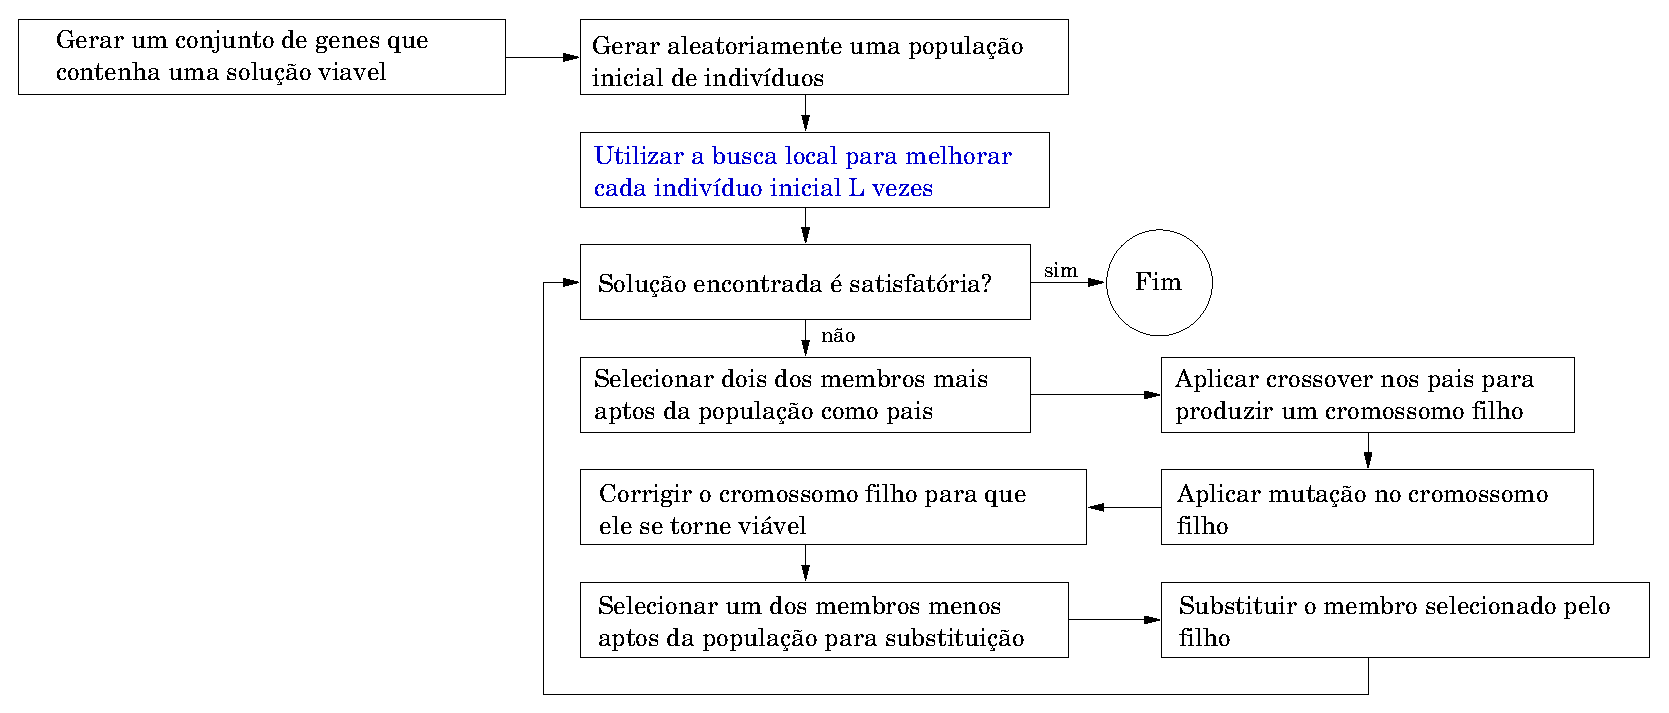
\includegraphics[scale=0.6]{fig/genetic.eps}
		\caption{Fluxograma mostrando o funcionamento do algoritmo genético híbrido proposto. O quadro 
		em azul representa uma novidade com relação ao algoritmo usual de~\cite{beasley96,kornilakis02},
		inspirado na heurística GRASP, resultando em um ganho considerável de qualidade e performance.}
		\label{fig:genetico}
	\end{center}
\end{figure}

%%%%%%%%%%%%%%%%%%%%%%%%%%%%%%%%%%%%%%%%%%%%%%%%%%%%%%%%%%%%%%%%%%%%%%%%%%%%%%%%%%%%%%%%%%%%%%%%%%%%

\section{Geração de Colunas}
\label{sec:metodos_colunas}

A solução do PDV pode ser obtida exatamente através de um algoritmo {\it branch-and-bound} que
envolve a resolução de uma relaxação linear do PLI associado em cada nó da árvore enumerativa do
procedimento. O grande número de variáveis torna difícil a resolução do programa linear relaxado
usando método tradicionais, como o algoritmo Simplex. Isso motiva a utilização de técnicas que não
requerem enumeração explícita de toda a matriz das restrições, tais como a geração de colunas.

Dantzig e Wolfe~\cite{dantzig60} desenvolveram um técnica para resolver PL grandes e especialmente
estruturados. Tal técnica consiste na solução alternada de um problema coordenador mestre restrito e
de subproblemas lineares menores. Métodos de geração de colunas, baseados no princípio de
decomposição de Dantzig e Wolfe, aproveitam-se do fato de que não é necessário ter disponível toda a
matriz de restrições durante o processamento. As colunas devem ser geradas apenas quando necessário.

Considere o seguinte programa linear, denotado por Problme Mestre (PM), onde o número de variáveis,
ou colunas, $n$, é muito grande:
%
\begin{eqnarray*} 
	\text{minimizar} && c_1 x_1 + c_2 x_2 + \ldots + c_n x_n \\
	\text{sujeito à} && a_{i1} x_1 + a_{i2} x_2 + \ldots + a_{in} x_n = b_i 
	\ev \;\; i = 1, \ldots, m \\
		               && x_j \geq 0 \ev \;\; j = 1, \ldots, n \ep 
\end{eqnarray*} 
%
Podemos assumir, sem perda de generalidade, que certas variáveis, 
$x_{\ell+1}, x_{\ell+2}, \ldots, x_{n}$, são não-básicas. Assim, podemos definir um problema
restrito, chamado de Problema Restrito Mestre (PRM), da seguinte forma:
%
\begin{eqnarray*} 
	\text{minimizar} && c_1 x_1 + c_2 x_2 + \ldots + c_\ell x_\ell \\
	\text{sujeito à} && a_{i1} x_1 + a_{i2} x_2 + \ldots + a_{in} x_n = b_i 
	\ev \;\; i = 1, \ldots, m \\
		               && x_j \geq 0 \ev \;\; j = 1, \ldots, \ell \ep 
\end{eqnarray*}

Note que a solução do PRM, se viável, pode ser ótima para o PM. Sejam $\pi_1 \, \pi_2, \ldots, 
\pi_m$ as variáveis duais ótimas para o PRM. O custo reduzido da variável $j$ é definido por
%
\begin{equation*}
\bar{c}_j = c_j - \sum_{i=1}^m \pi_i a_{ij} \ep
\end{equation*}
%
Da teoria de programação linear, sabemos que se o custo reduzido de cada variável é não-nulo, então
a solução do PRM é ótima para o PM. Portanto, para se determinar se o ótimo do PM foi atingido,
o seguinte Subproblema (denotado por SP) deve ser resolvido:
%
\begin{equation} \label{eq:pricing}
	w^\ast = \min_{j = 1, \ldots, n} \left[ c_j - \sum_{i=1}^m \pi_i a_{ij} \right] \ev
\end{equation}
%
Se $w^\ast \geq 0$ a solução do PRM é ótima para o PM. Caso contrário, se $w^\ast < 0$, a coluna 
$k$, tal que $\bar{c}_k < 0$ é identificada e adicionada ao PRM. O PRM é resolvido novamente com 
essa nova coluna, e todo o processo é repetido até que nenhum variável com custo reduzido negativo
seja encontrada. O problema (\ref{eq:pricing}) é conhecido como {\it pricing problem}.

Especializando o procedimento de geração de colunas para o PDV, observamos que o SP
(\ref{eq:pricing}) pode ser resolvido usando um procedimento de caminho mais curto na rede de voos
correspondente. Associamos a variável dual $\pi_i$ para cada nó correspondente ao voo $i$. Rodando o
procedimento de caminho mais curto entre fonte e sorvedouro para cada base de tripulação, usando
arcos com custos iguais aos custos reduzidos, a viagem de menor custo reduzido pode ser encontrada.
Se $w^\ast$ (o custo reduzido mínimo da equação (\ref{eq:pricing})) é não-negativo, então todas as
viagens tem custo reduzido não-negativo e portanto o algoritmo de geração de coluna pode ser
terminado. De forma contrária, viagens de custos reduzidos negativos são identificadas e adicionadas
como colunas ao problema mestre restrito, de forma que a próxima iteração do algoritmo pode ser
executada (confira a Figura~\ref{fig:cg}).

\begin{figure}[htbp]
	\begin{center}
		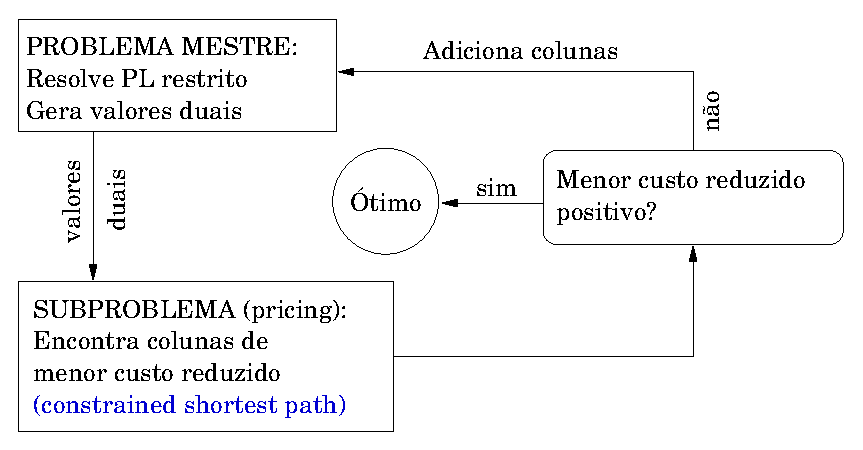
\includegraphics[scale=0.6]{fig/cg.eps}
		\caption{Fluxograma mostrando o funcionamento do procedimento de geração de colunas.
		O {\it princing problem} é traduzido em um problema de caminho mais curto com restrições.}
		\label{fig:cg}
	\end{center}
\end{figure}

O procedimento de busca do caminho mais curto na rede de voos deve levar em consideração a 
viabilidade dos caminhos percorridos. Recaímos, portanto, em um problema de caminho mais curto
com restrições.

Problemas simples (ou sem restrições) de caminho mais curto envolvem apenas a determinação do 
caminho de menor custo sem considerações adicionais e podem ser resolvidos em tempo polinomial. 
Problemas de caminho mais curto com restrições podem levar tempo exponencial.

Para ilustração, consire o problema comum de caminho mais curto, onde um rótulo em cada nó dá o 
comprimento do caminho mais curto atual a partir da fonte até o dado nó. Como cada rótulo contém
apenas um custo, ele pode, sem ambiguidade, dominar ou ser dominado por outro rótulo: um rótulo mais
barato domina um rótulo mais caro.

No caso de problemas de caminho mais curto com restrições, em cada nó pode haver um conjunto de 
rótulos, cada qual correspondendo a um caminho e nenhum deles sendo dominante. Tal conjunto de 
rótulos é dito {\it eficiente}. Um rótulo pode dominar outro rótulo apenas se ele tiver custo
menor e for menos restrito com relação a todos os parâmetros que governam a viabilidade dos 
caminhos. Suponha em um nó que nenhum dos rótulos possa dominar os outros, então todos eles devem 
ser armazenados. Como teoricamente pode haver um número exponencial de caminhos no grafo, um número
exponencial de rótulos também pode existir, fazendo, portanto, com que o algoritmo leve um tempo
exponencial para ser executado.

A Figura~\ref{fig:shortest_path} pode ser utilizada para demonstrar o procedimento de solução
adotado para resolver o problema de caminho mais curto com restrições. Suponha que o custo de um
caminho seja a soma do segundo parâmetro de todas as arestas que constituem o caminho, e que o
primeiro parâmetro seja um recurso sendo consumido ao se utilizar a aresta. Gostaríamos de encontrar
o caminho de custo mínimo entre os nós $s$ e $t$ que satisfaça a restrição de que o total de
recursos utilizados no caminho seja menor ou igual a 4. O algoritmo procede com uma busca em 
profundidade, efetuando um cheque de dominância entre os rótulos de cada nó atingido.

\begin{figure}[htbp]
	\begin{center}
		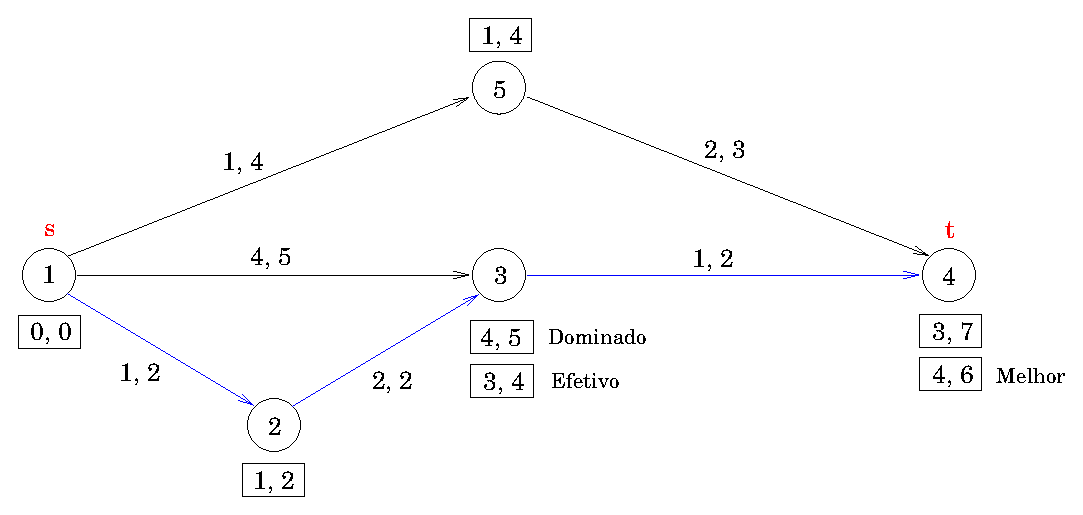
\includegraphics[scale=0.6]{fig/shortest_path.eps}
		\caption{Caminho mais curto com restrições entre os nós $s$ e $t$: $1 \to 2 \to 3 \to 4$.
		O primeiro parâmetro nas arestas indica o custo e o segundo o valor de um recurso a ser
    consumido. A restrição imposta é de que o total de recursos utilizados pelo caminho seja 
		$\leq 4$.}
		\label{fig:shortest_path}
	\end{center}
\end{figure}

\zerar
\chapter{Resultados e Discussão}
\label{cap:resultados}

Em nosso estudo utilizamos os pacotes de otimização GLPK (GNU Linear Programming Kit) e Cplex da
IBM. Os resultados finais, entretanto, são baseados apenas na utilização da ferramenta Cplex, uma
vez que a mesma provou ser mais eficiente. Além disso, o otimizador Cplex pôde ser utilizado
diretamente a partir de nosso código, alimentando o modelo gerado através da API Java fornecida pela
IBM. Por outro lado, como o GLPK não fornece API apropriada, sua utilização se limitou a geração do
modelo em arquivo (formato mps) e posterior execução do otimizador em um processo separado, sendo
necessário realizar um {\it parsing} no arquivo de saída gerado para obtenção dos resultados.

Implementamos os métodos de solução do PDV descritos no Capítulo~\ref{cap:heuristicas}. Os 
parâmetros utilizados, que garantem a legalidade das viagens geradas, são apresentados na
Tabela~\ref{tab:parametros} e baseiam-se na legislação brasileira para aviação comercial regular.

Todos os testes foram realizados em um computador utilizando um processador Intel Core~i3 64~bits, 
com 4~Gb de memória RAM, rodando o sistema operacional MacOS~10.6. Toda a implementação foi escrita 
em Java (JDK~1.6.33).

\begin{table}
	\begin{center}
		\begin{tabular}{|l|l|l|}
			\hline 
			\bf Parâmetro & \bf Descrição & \bf Valor \\
			\hline \hline 
			\verb|MAX_LEGS| & Máximo de pernas por jornada & 5 \\ \hline
			\verb|MAX_TRACKS| & Máximo de trocas de aeronave por jornada & 2 \\ \hline
			\verb|MAX_FLIGHT_TIME| & Total máximo de voo por jornada & 9,5 h \\ \hline
			\verb|MAX_DUTY_TIME| & Duração máxima de uma jornada & 11,5 h \\ \hline
			\verb|MIN_SIT_TIME| & Tempo mínimo de conexão & 30 min \\ \hline
			\verb|MAX_SIT_TIME| & Tempo máximo de conexão & 120 min \\ \hline
			\verb|BRIEFING_TIME| & Tempo para o {\it briefing} & 0 min \\ \hline
			\verb|DEBRIEFING_TIME| & Tempo para o {\it debriefing} & 0 min \\ \hline
			\verb|MIN_REST_TIME| & Tempo mínimo de repouso & 12 h \\ \hline
			\verb|MAX_REST_TIME| & Tempo máximo de repouso & 36 h \\ \hline
			\verb|MAX_DUTIES| & Máximo de jornadas por viagem & 2, 3 ou 4 \\ \hline
			\end{tabular} 
			\caption{Parâmetros utilizados na geração das viagens.}
			\label{tab:parametros}
	\end{center}
\end{table}

%%%%%%%%%%%%%%%%%%%%%%%%%%%%%%%%%%%%%%%%%%%%%%%%%%%%%%%%%%%%%%%%%%%%%%%%%%%%%%%%%%%%%%%%%%%%%%%%%%%%

\section{Análise Preliminar}
\label{sec:preliminar}

O objetivo desta análise preliminar foi definir o limite de utilização do procedimento de geração
de viagens e do otimizador na resolução exata do modelo {\it set partition} (\ref{eq:sppv}).
Com essa finalidade, construímos alguns gráficos que relacionam o tempo de geração e otimiazação 
utilizado em nossa implementação, em função do número de etapas da entrada do problema.

Para estudar a influência do número de pernas isoladamente, restringimos a entrada apenas para um
conjunto de voos entre duas localidades, São Paulo (CGH) e Rio de Janeiro (SDU), considerando os
trechos diárias oferecidos na ponte-aérea pela companhia aérea Gol. Um total de 62 pernas 
(31 de CGH para SDU e 31 de SDU para CGH) representam a instância global de entrada.

Vale observar que o caso da ponte-aérea é um pouco atípico no sentido de que representa um malha 
muito densa de voos: muitas etapas são oferecidas de ida e volta num curto intervalo de tempo, 
criando muitas conexões legais (arcos) entre os nós da rede de voos gerada. Com isso, o número
de viagens dado pela procedimento de busca no grafo explode rapidamente.

O gráfico da Figura~\ref{fig:pairings} mostra o número de viagens geradas em função do número de
etapas na ponte-aérea. As viagens foram geradas para a base CGH. São apresentadas três curvas, uma
para cada valor do parâmetro \verb|MAX_DUTIES| (2, 3 e 4). Observe a escala logarítmica do eixo
vertical. O comportamento praticamente linear das curvas indica um crescimento exponencial do número
de viagens que podem ser geradas. Observe ainda que a taxa de crescimento é maior quanto maior o
número máximo de jornadas permitidas, já que nesse caso permite-se um número muito maior de
combinações. Para \verb|MAX_DUTIES| = 4, encontrou-se um número da ordem de $10^8$ viagens com
apenas 36 pernas.

\begin{figure}[htp]
	\begin{center}
		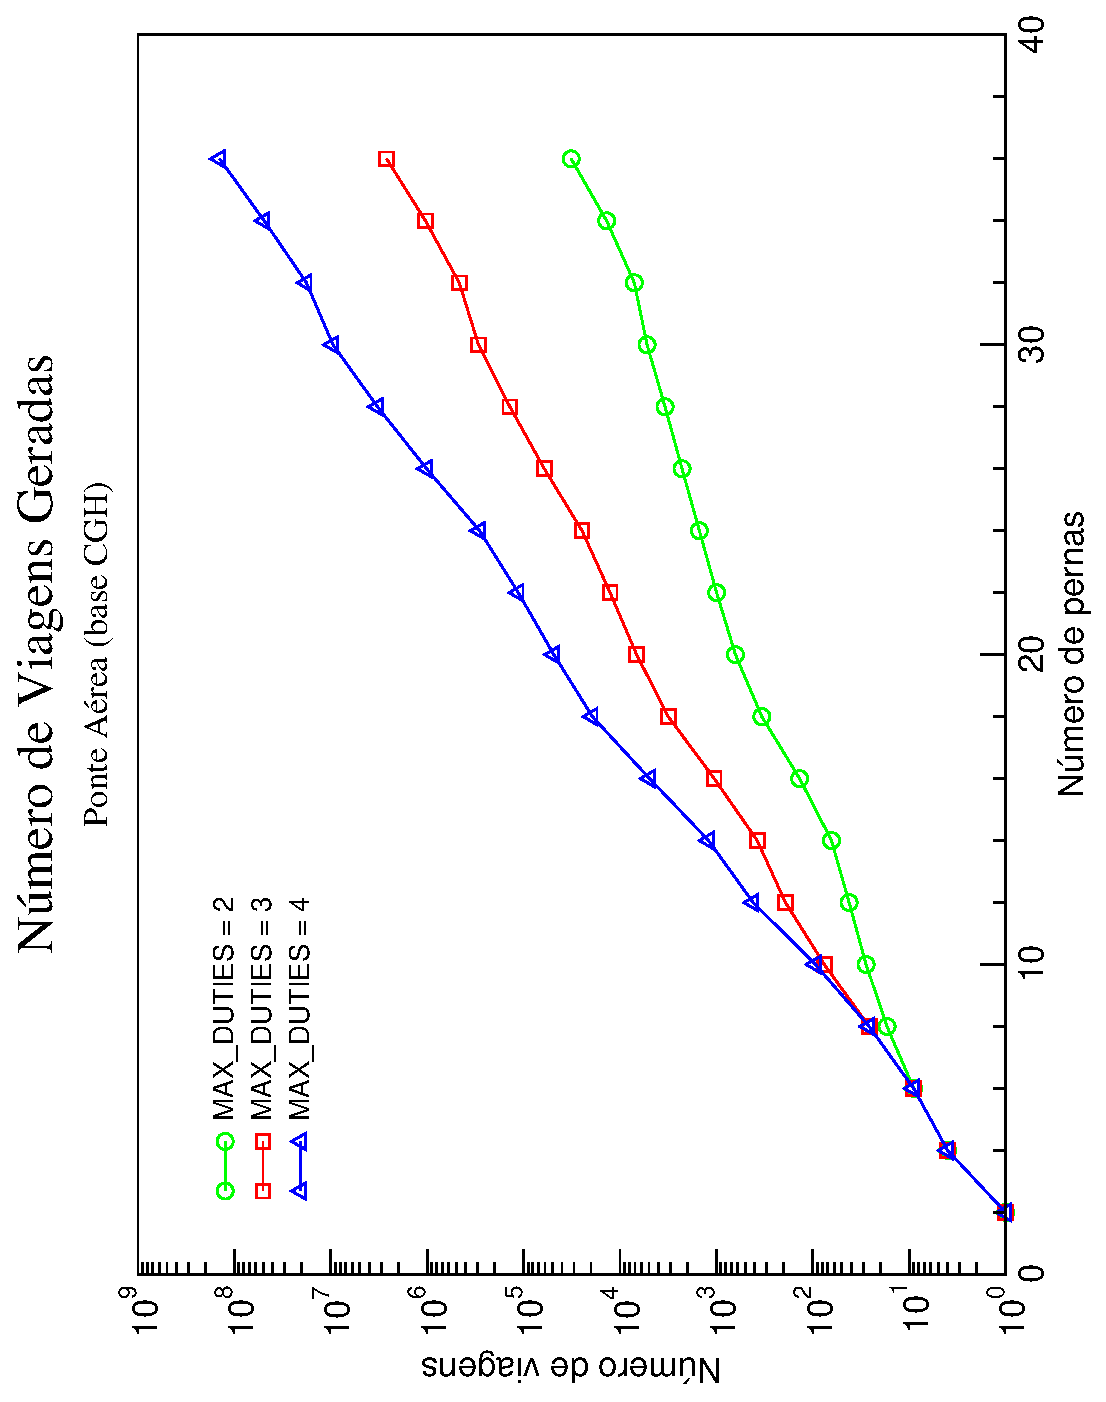
\includegraphics[scale=0.45,angle=-90]{fig/number_of_pairings.eps}
		\caption{Número de viagens geradas em função do número de pernas utilizadas na construção da
		rede de voos.}
		\label{fig:pairings}
	\end{center}
\end{figure}

O consumo de tempo gasto pelo algoritmo de busca em profundidade também foi medido em função do 
número de pernas. Os resultados são apresentados na Figura~\ref{fig:generation}. O comportamento das
curvas indicam também um crescimento exponencial do tempo gasto pelo algoritmo, ainda que ele seja
executado de forma rápida (para \verb|MAX_DUTIES| = 4, encontrou-se um tempos da ordem de $10^4$~ms 
para 36 pernas).

\begin{figure}[htb]
	\begin{center}
		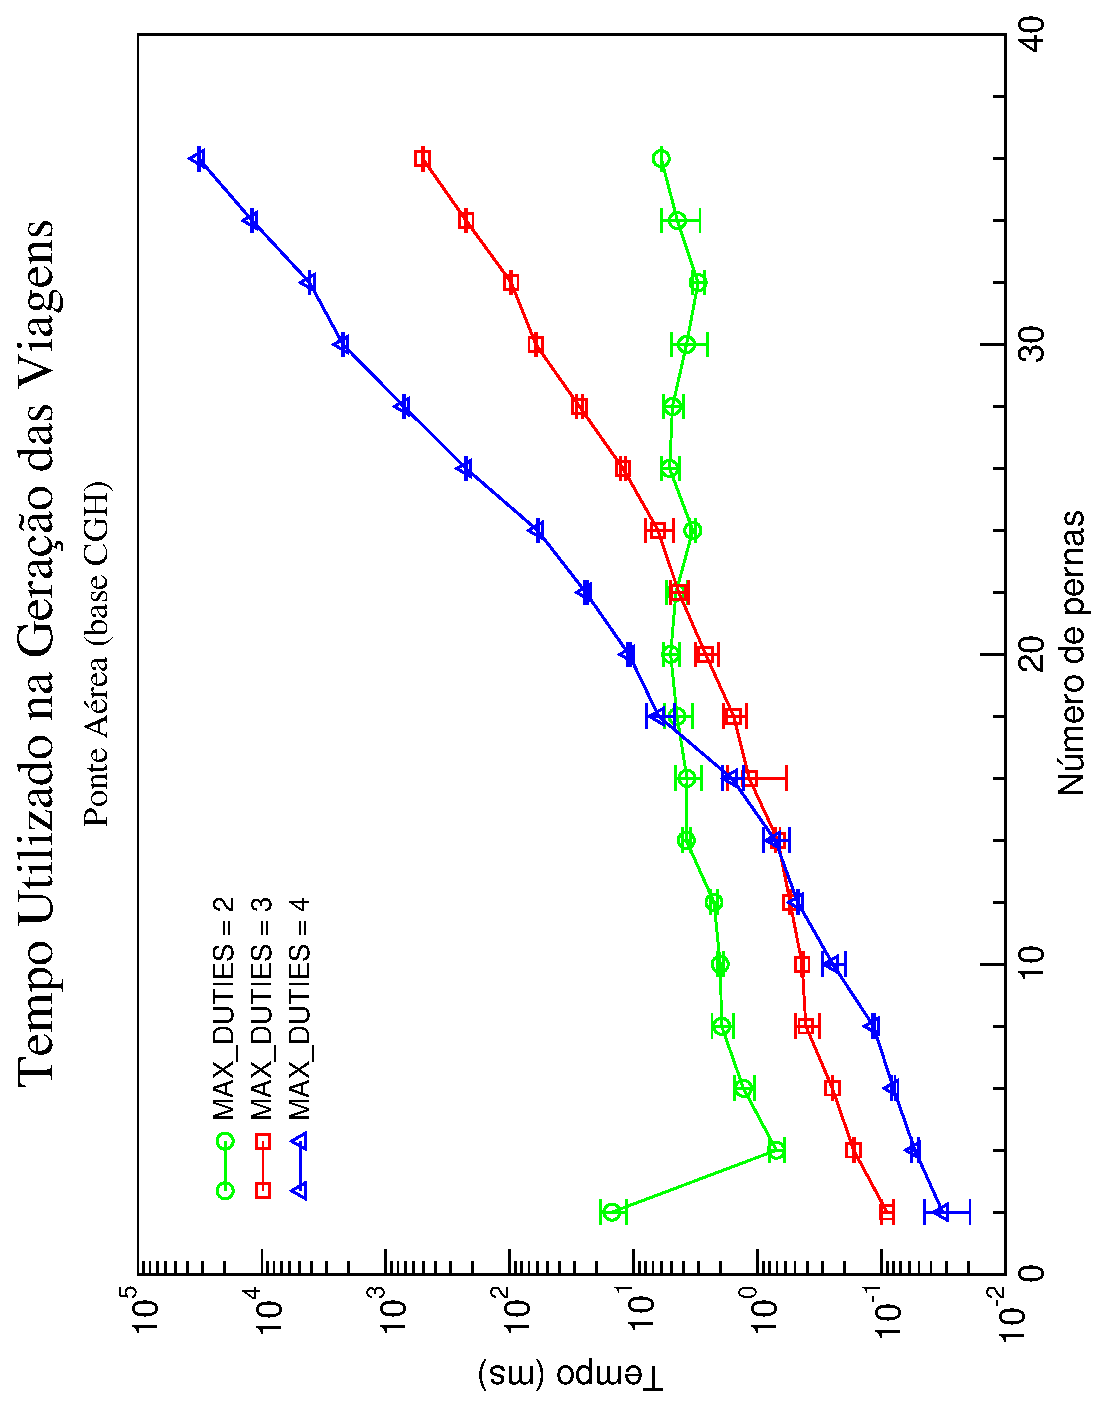
\includegraphics[scale=0.45,angle=-90]{fig/generation_time.eps}
		\caption{Tempo gasto na geração das viagens em função do número de pernas utilizadas na 
		construção da rede de voos. São apresentados valor médio $\pm$ desvio-padrão, considerando 5 
		medidas para cada ponto. O primeiro ponto da curva verde encontra-se um pouco fora provavelmente
		devido a algum transiente da máquina, visto que ele foi o primeiro a ser processado.}
		\label{fig:generation}
	\end{center}
\end{figure}

O tempo gasto pelo otimizador GLPK para resolver o modelo proposto é apresentado no gráfico da 
Figura~\ref{fig:glpk}. Mais uma vez, observa-se um crescimento exponencial muito forte (note a 
escala logarítmica do eixo vertical) em função do número de etapas considerado. A 
Figura~\ref{fig:cplex} mostra os resultados obtidos para o otimizador Cplex. 

\begin{figure}[htb]
	\begin{center}
		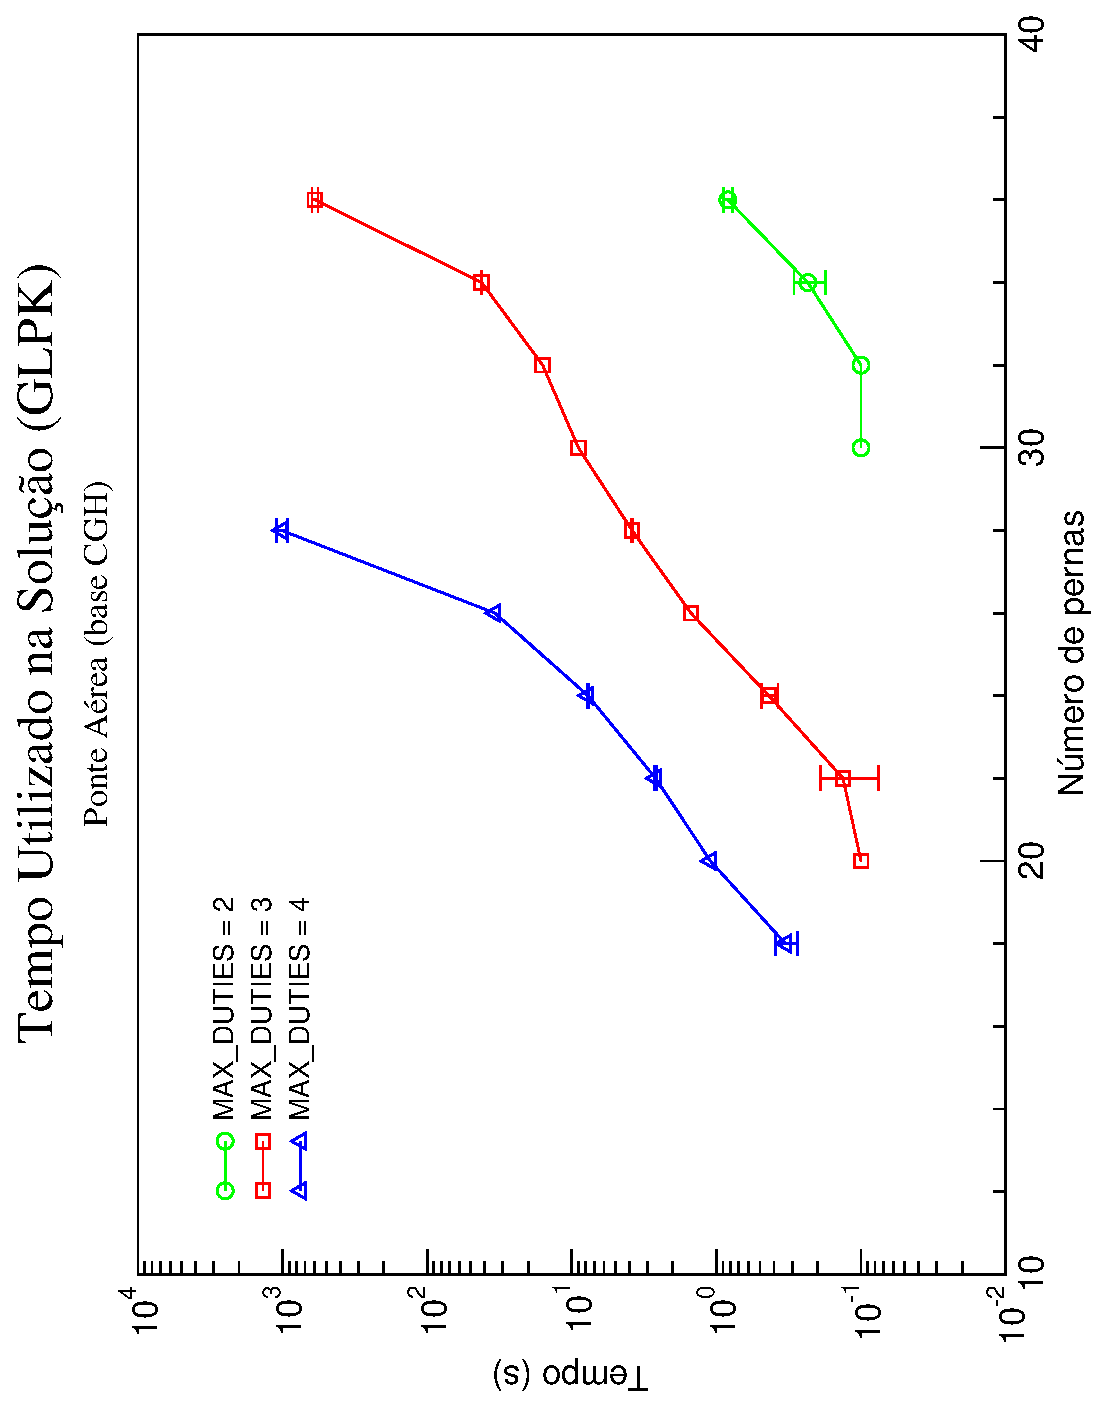
\includegraphics[scale=0.45,angle=-90]{fig/glpk_solution_time.eps}
		\caption{Tempo utilizado pelo otimizador GLPK na obtenção de uma solução inteira, em função do 
		número de etapas. São apresentados valor médio $\pm$ desvio-padrão, considerando 3 medidas para 
		cada ponto. Valores medidos com tempo de execução de 0,0~s não são apresentados (número pequeno 
		de pernas). Os últimos pontos da curva azul não puderam ser estimados, mesmo após algumas horas 
		de processamento.}
		\label{fig:glpk}
	\end{center}
\end{figure}

\begin{figure}[htb]
	\begin{center}
		\includegraphics[scale=0.45,angle=0]{fig/cplex_solution_time.eps}
		\caption{Resultados obtidos para o otimizador Cplex. Valem as mesmas observações feitas na 
		legenda da Figura~\ref{fig:glpk}.}
		\label{fig:cplex}
	\end{center}
\end{figure}

%%%%%%%%%%%%%%%%%%%%%%%%%%%%%%%%%%%%%%%%%%%%%%%%%%%%%%%%%%%%%%%%%%%%%%%%%%%%%%%%%%%%%%%%%%%%%%%%%%%%

\section{Instâncias}
\label{sec:instancias}

Os métodos heurísticos implementados foram testados em dados reais dados pelas instâncias listadas
na tabela~\ref{tab:instancias}. Os dados se referem a voos diários oferecidos no passado pelas
companhias Gol e WebJet. 

Na tabela são indicados o nome da instância, a companhia a qual pertence, a frota de aeronaves a que
se refere, o número de etapas e o número de trilhos. O trilho identifica o conjunto de etapas que
uma determinada aeronave da frota deve executar diariamente. No caso de uma frota com $k$ aeronaves,
deverão ser fornecidos $k$ trilhos distintos.

A instância PA\_62 se refere a voos na ponte-aérea estudados na análise preliminar. A instância mais
difícil se refere à 73G\_340, com 340 etapas diárias e 40 trilhos de aeronaves.

\begin{table}[htb]
	\begin{center} 
		\begin{tabular}{|l|l|l|l|l|}
			\hline 
			{\bf Instância} & {\bf Cia} & {\bf Frota} & {\bf Etapas} & {\bf Trilhos} \\ 
			\hline \hline
			73H\_26 & Gol & 737-800 & 26 & 5 \\ 
			738\_48 & WebJet & 737-800 & 48 & 7 \\ 
			733\_92 & WebJet & 737-300 & 92 & 12 \\
			73G\_340 & Gol & 737-700 & 340 & 40 \\
			PA\_62 & Gol & 737-800S & 62 & 6 \\ \hline
		\end{tabular}
		\caption{Caracterização das instâncias utilizadas para testes em nosso estudo.}
		\label{tab:instancias}
	\end{center}
\end{table}

%%%%%%%%%%%%%%%%%%%%%%%%%%%%%%%%%%%%%%%%%%%%%%%%%%%%%%%%%%%%%%%%%%%%%%%%%%%%%%%%%%%%%%%%%%%%%%%%%%%%

\section{Soluções Exatos}
\label{sec:solucoes_exatas}

Apenas três instâncias (pequenas) puderam ser resolvidas exatamente pela solução do modelo {\it set
partition} (\ref{eq:sppv}), com um tempo de processamento aceitável. A descrição dos problemas é
apresentada na Tabela~\ref{tab:problemas}.

\begin{table}[htb]
	\begin{center} 
		\begin{tabular}{|c|c|c|}
			\hline 
			{\bf Problema} & {\bf Instância} & {\bf Bases} \\ 
			\hline \hline
			P1 & 73H\_26 & GRU \\ 
			P2 & 738\_48 & GRU e GIG \\ 
			P3 & 733\_92 & GRU, GIG e POA \\ \hline
		\end{tabular}
		\caption{Caracterização dos problemas resolvidas exatamente através dos modelos 
		{\it set partition} e {\it set cover}. GRU = São Paulo, GIG = Rio de Janeiro e POA = Porto
    Alegre.}
		\label{tab:problemas}
	\end{center}
\end{table}

Na resolução dos problemas, foram utilizados os parâmetros da Tabela~\ref{tab:parametros}. Além
disso, limitou-se a 2 o número máximo de trocas de aeronaves por jornada. Com isso, forçamos a
tripulação acompanhar, na medida do possível, o trilho percorrido pela aeronave, reduzindo a
possibilidade de conexões em cada localidade. Naturalmente os tempos de conexão serão reduzidos,
tornando as viagens geradas mais baratas e diminuindo o número total de variáveis geradas. Além
disso, esse procedimento torna a solução mais robusta, uma vez que o atraso de uma aeronave não
acarretará atraso na saída de outro voo que dependa daquela aeronave na troca.

O custo de uma viagem foi calculado como sendo o tempo ``ocioso'' relativo no qual o tripulante está 
trabalhando mas não está voando, ou seja, pela diferença entre o tempo total de uma viagem, menos o 
tempo total de voo efetuado, descontando ainda os tempos mínimos regulamentares de conexão entre 
pernas e de descanso entre jornadas, dividido pelo tempo total de voo. Esse custo avalia de forma 
relativa a produtividade de uma viagem, o qual deve ser minimizado na solução final.

Os resultados obtidos são apresentados e resumidos na Tabela~\ref{tab:resultados}. Nela são 
indicadas a instância resolvida, o número total de variáveis geradas, o número de viagens na 
solução, o custo da solução e o tempo de processamento do otimizador (Cplex).

\begin{table}[htb]
	\begin{center} 
		\begin{tabular}{|c|c|c|c|c|}
			\hline 
			{\bf Problema} & {\bf Variáveis} & {\bf Viagens} & {\bf Custo} & {\bf Tempo (s)} \\ 
			\hline \hline
			P1 & 180 & 6 & 6,952 & $< 1$ \\ 
			P2 & 66411 & 6 & 6,436 & 3,75 \\
			P3 & 1023818 & 11 & 6,942 & 170,86 \\ \hline
		\end{tabular}
		\caption{Resultados obtidos na geração e otimização de viagens para os problemas consideradas.}
		\label{tab:resultados}
	\end{center}
\end{table}

As mesmas instâncias 73H\_26, 738\_48, 733\_92 também foram resolvidas utilizando o modelo {\it set
cover} (\ref{eq:scpdv}), o qual admite a existência de {\it deadheading}. Os resultados obtidos
foram idênticos aos listados na Tabela~\ref{tab:resultados}. Em particular, todas as variáveis
artificiais $y_i$ receberam valor zero na solução final, indicando a não necessidade de {\it
deadheading}.

%%%%%%%%%%%%%%%%%%%%%%%%%%%%%%%%%%%%%%%%%%%%%%%%%%%%%%%%%%%%%%%%%%%%%%%%%%%%%%%%%%%%%%%%%%%%%%%%%%%%

\section{Uma Solução Explícita}
\label{sec:solucao_explicita}

Para tornar mais concreto a entrada e a saída do problema, apresentamos na Tabela~\ref{tab:73H_26} o
conjunto de etapas referentes a instância 73H\_26\footnote{Não há problema de confidencialidade nos
dados apresentados, uma vez que os mesmos se referem a dados do passado liberados pela companhia
aérea.}. A mesma representa 26 trechos oferecidos diariamente pela companhia aérea Gol para uma
frota especial de 5 aeronaves B737-800. Para cada etapa são fornecidos o seu número, aeroporto de
origem, aeroporto de destino, horário local de decolagem (DEP) e horário local de pouso (ARR) e o
trilho correspondente.

Na Tabela~\ref{tab:pairings} listamos as 6 viagens geradas como solução do problema de otimização.
Cada etapa na tabela apresenta o número do voo, origem e destino, horário local de decolagem e 
pouso, e o trilho executado. O custo final resultante foi de 6,952, para um total de 180 variáveis 
geradas, considerando a base GRU (São Paulo). Observe a presença de uma viagem bate-volta (4),
bem como uma viagem de 3 dias de duração (5).

\begin{table}[htb]
	\begin{center}
		\scalebox{0.73}{
		\begin{tabular}{|cccccc|}
			\hline 
			{\bf Número} & {\bf Origem} & {\bf Destido} & {\bf DEP} & {\bf ARR} & {\bf Trilho} \\
			\hline \hline
			7625 & GRU &	GIG	 &  07:00	 &  08:00  & 1 \\
			7622 & GIG &	GRU	 &  09:00	 &  09:55	 & 1 \\
			7622 & GRU &	CCS	 &  11:00	 &  15:30	 & 1 \\
			7622 & CCS &	AUA	 &  16:10	 &  17:55	 & 1 \\
			7623 & AUA &	CCS	 &  21:20	 &  22:05	 & 1 \\
			7623 & CCS &	GRU	 &  22:45	 &  06:00	 & 1 \\
			1841 & CWB &	GRU	 &  07:52	 &  08:55	 & 2 \\
			1902 & GRU &	NAT	 &  11:00	 &  14:20	 & 2 \\
			1903 & NAT &	GRU	 &  15:30	 &  19:10	 & 2 \\
			1704 & GRU &	MAO	 &  21:15	 &  00:10	 & 2 \\
			1798 & GRU &	REC	 &  08:05	 &  11:21	 & 3 \\
			1149 & REC &	GRU	 &  12:04	 &  15:30	 & 3 \\
			7680 & GRU &	AEP	 &  18:25	 &  21:15	 & 3 \\
			7681 & AEP &	GRU	 &  22:40	 &  01:30	 & 3 \\
			1705 & MAO &	GRU	 &  03:42	 &  08:35	 & 4 \\
			1766 & GRU &	CWB	 &  09:20	 &  10:16	 & 4 \\
			1846 & CWB &	GRU	 &  11:13	 &  12:15	 & 4 \\
			7480 & GRU &	ASU	 &  13:05	 &  13:50	 & 4 \\
			1847 & GRU &	CWB	 &  18:10	 &  19:20	 & 4 \\
			1767 & CWB &	GRU	 &  20:56	 &  21:50	 & 4 \\
			1566 & GRU &	CWB	 &  22:35	 &  23:30	 & 4 \\
			7481 & ASU &	GRU	 &  14:30	 &  17:25	 & 4 \\
			7678 & GRU &	AEP	 &  08:00	 &  10:50	 & 5 \\
			7679 & AEP &	GRU	 &  11:50	 &  14:35	 & 5 \\
			7658 & GRU &	EZE	 &  15:15	 &  18:15	 & 5 \\
			7659 & EZE &	GRU	 &  20:35	 &  23:25	 & 5 \\ \hline
	\end{tabular}}
	\caption{Dados que caracterizam a instância 73H\_26.}
	\label{tab:73H_26}
	\end{center}
\end{table}


\begin{table}[htb]
	\begin{center}
		\scalebox{0.73}{
		\begin{tabular}{|c|c|ccccc|}
			\hline
			{\bf Viagem} & {\bf Jornada} & \multicolumn{5}{|c|}{\bf Etapa} \\ \hline \hline
			\multirow{6}{*}{1} & \multirow{4}{*}{1}  
			  & 7625 & GRU-GIG & 07:00 & 08:00 & 001 \\
			& & 7622 & GIG-GRU & 09:00 & 09:55 & 001 \\
			& & 7622 & GRU-CCS & 11:00 & 15:30 & 001 \\
			& & 7622 & CCS-AUA & 16:10 & 17:55 & 001 \\ \cline{2-7}
			                       & \multirow{2}{*}{2}
				& 7623 & AUA-CCS & 21:20 & 22:05 & 001 \\
			& &	7623 & CCS-GRU & 22:45 & 06:00 & 001 \\ \hline \hline
			\multirow{2}{*}{2} & \multirow{2}{*}{1}  		
				& 1902 & GRU-NAT & 11:00 & 14:20 & 002 \\
			& & 1903 & NAT-GRU & 15:30 & 19:10 & 002 \\ \hline \hline
			\multirow{2}{*}{3} & \multirow{1}{*}{1}  		
				& 1704 & GRU-MAO & 21:15 & 00:10 & 002 \\ \cline{2-7}
                           	& \multirow{1}{*}{2}
				&	1705 & MAO-GRU & 03:42 & 08:35 & 004 \\ \hline \hline
			\multirow{2}{*}{4} & \multirow{2}{*}{1}  		
				& 1798 & GRU-REC & 08:05 & 11:21 & 003 \\
			& & 1149 & REC-GRU & 12:04 & 15:30 & 003 \\ \hline \hline			
			\multirow{10}{*}{5} & \multirow{3}{*}{1}  
				&	1847 & GRU-CWB & 18:10 & 19:20 & 004 \\
			& &	1767 & CWB-GRU & 20:56 & 21:50 & 004 \\
			& &	1566 & GRU-CWB & 22:35 & 23:30 & 004 \\ \cline{2-7}
                           		& \multirow{4}{*}{2}
				&	1841 & CWB-GRU & 07:52 & 08:55 & 002 \\
			&	&	1766 & GRU-CWB & 09:20 & 10:16 & 004 \\
			&	&	1846 & CWB-GRU & 11:13 & 12:15 & 004 \\
			&	&	7480 & GRU-ASU & 13:05 & 13:50 & 004 \\ \cline{2-7}
                           		& \multirow{3}{*}{3}
				&	7481 & ASU-GRU & 14:30 & 17:25 & 004 \\
			&	&	7680 & GRU-AEP & 18:25 & 21:15 & 003 \\
			&	&	7681 & AEP-GRU & 22:40 & 01:30 & 003 \\ \hline \hline
			\multirow{4}{*}{6} & \multirow{3}{*}{1}  
				& 7678 & GRU-AEP & 08:00 & 10:50 & 005 \\
			& & 7679 & AEP-GRU & 11:50 & 14:35 & 005 \\
			&	& 7658 & GRU-EZE & 15:15 & 18:15 & 005 \\ \cline{2-7}
                           	 & \multirow{1}{*}{2}
				& 7659 & EZE-GRU & 20:35 & 23:25 & 005 \\ \hline
		\end{tabular}}
		\caption{Conjunto de viagens obtido como solução ótima da instância 73H\_26.}
		\label{tab:pairings}
	\end{center}
\end{table}

%%%%%%%%%%%%%%%%%%%%%%%%%%%%%%%%%%%%%%%%%%%%%%%%%%%%%%%%%%%%%%%%%%%%%%%%%%%%%%%%%%%%%%%%%%%%%%%%%%%%

\section{Aplicação das Heurísticas}
\label{sec:aplicacao_heuristicas}

Como esperado, os métodos exatos mostraram-se ineficientes para instâncias grandes ou até mesmo para
uma instância pequena de ponte-aérea. Apesar de não garantir solução ótima, os métodos aproximados
apresentaram soluções aceitáveis, em alguns casos ótimas, em tempos de execução pequenos. A seguir
apresentaremos os resultados específicos de cada método implementado.

Todos os testes forma realizados nas instâncias da Tabela~\ref{tab:instancias}, considerando apenas
a base GRU para geração de viagens. O número máximo de jornadas foi escolhido 4, menos no caso da
ponte-aérea (PA\_62), onde consideramos o valor 2 (no máximo um pernoite).

A função de custo utilizada para cada viagem foi uma que buscava maximizar a relação de horas de voo
por horas de jornada. Buscamos com isso viagens com jornadas produtivas para os tripulantes. Mais
especificamente, se $F_j$ é o tempo total de voo de uma viagem $j$ e $D_j$ o seu tempo total de
jornada, então $c_j = D_j / F_j$.

%%%%%%%%%%%%%%%%%%%%%%%%%%%%%%%%%%%%%%%%%%%%%%%%%%%%%%%%%%%%%%%%%%%%%%%%%%%%%%%%%%%%%%%%%%%%%%%%%%%%

\subsection{Valores}
\label{sec:valores}

A Tabela~\ref{tab:comparacao} mostra os resultados do processo de otimização para as três
heurísticas. São apresentados tempo de processamento em segundos (CPU) e valor da função objetivo
(OBJ) para a melhor solução encontrada. O valor de DH entre parênteses indica o número de etapas
sobrecobertas na solução ({\it deadheads}). A tabela ainda explora os resultados para três valores
dos parâmetros $k$ e $L$ dos métodos de busca local e algoritmo genético híbrido, respectivamente.

O método de geração de colunas fornece um limitante inferior para o custo da solução, já que resolve
de forma ótima a relaxação linear do problema. O custo obtido pelos demais métodos é expresso em
\% com relação ao valor desse limitante inferior.

\begin{table}[ht]
\begin{center}
\scalebox{0.72}{
\begin{tabular}{cc|c|c|c|c|c|c|c|c|c|c|}
	\cline{3-12}
	& &
	\multicolumn{2}{|c|}{\bf 73H\_26} & 
	\multicolumn{2}{|c|}{\bf 738\_48} & 
	\multicolumn{2}{|c|}{\bf 733\_92} & 
	\multicolumn{2}{|c|}{\bf 73G\_340} & 
	\multicolumn{2}{|c|}{\bf PA\_62} \\
	\cline{3-12}
	& & OBJ (DH) & CPU & OBJ (DH) & CPU & OBJ (DH) & CPU & OBJ (DH) & CPU & OBJ (DH) & CPU \\

	\hline
	\multicolumn{2}{|c|}{GC} & 
	5,696 (0)  & 0,26  & 
	6,230 (0) & 0,54  & 
	10,973 (0) & 1,36  & 
	42,744 (0) & 54,02 & 
	10,103 (0) & 1,13 \\

	\hline
	\multicolumn{1}{|c|}{\multirow{3}{*}{BL}} 
	& $k = 2$ & 
	0\% (0) & 1,10   & 
	$>$100\% (116) & 1,22   & 
  $>$100\% (124) & 3,16   & 
	$>$100\% (654) & 208,44 & 
	$>$100\% (8) & 0,79 \\
	\multicolumn{1}{|c|}{} 
	& $k = 3$ &
	0\% (0) & 1,48    & 
	14,1\% (0) & 7,91    & 
	8,1\% (0) & 18,68   & 
	32,5\% (9) & 1303,53 & 
	87,7\% (0) & 1,31 \\
	\multicolumn{1}{|c|}{} 
	& $k = 4$ & 
	0\% (0) & 1,81 & 
	0\% (0) & 11,46 & 
	7,7\% (0) & 99,09 & 
	25,5\% (11) & 2182,31 & 
	0\% (0)   & 17,83 \\

	\hline
	\multicolumn{1}{|c|}{\multirow{3}{*}{AG}} 
	& $L = 1$ & 
	0\% (0) & 1,39 & 
	78,1\% (2) & 4,35 & 
	$>$100\% (9) & 8,30 & 
	$>$100\% (476) & 1074,97 & 
	56,2\% (0) & 4,31 \\
	\multicolumn{1}{|c|}{} 
	& $L = 5$ & 
	0\% (0) & 4,17 & 
	13,8\% (0) & 13,19 & 
	46,4\% (0) & 10,79 & 
	$>$100\% (208) & 763,19 & 
	36,2\% (0) & 13,99 \\
	\multicolumn{1}{|c|}{} 
	& $L = 10$ & 
	0\% (0) & 11,01 & 
	0\% (0) & 33,99 & 
	72,2\% (3)3 & 17,85 & 
	$>$100\% (78) & 482,10 & 
	30,5\% (0) & 27,50 \\
	\hline
\end{tabular}}
\caption{Resultados do processo de otimização para as três heurísticas: GC = geração de colunas,
BL = busca local e AG = algoritmo genético.}
\label{tab:comparacao}
\end{center}
\end{table}

A partir dos dados da Tabela~\ref{tab:comparacao}, faremos uma análise dos resultados para cada uma 
das heurísticas estudadas nas seções seguintes.

%%%%%%%%%%%%%%%%%%%%%%%%%%%%%%%%%%%%%%%%%%%%%%%%%%%%%%%%%%%%%%%%%%%%%%%%%%%%%%%%%%%%%%%%%%%%%%%%%%%%

\subsection{Busca Local}
\label{sec:resultados_busca}

O método de Busca Local revelou-se eficiente para todos os tamanhos de instância, produzindo
soluções ótimas para instâncias pequenas e médias, e próximas ao ótimo para instâncias grandes. O
número de viagens, $k$, escolhido por iteração deve ser definido {\it a priori}. 

A Figura~\ref{fig:ls_results} mostra a evolução do processo de otimização para cada um dos problemas
considerados e cada valore de $k$ escolhido.

\begin{figure}[htbp]
	\begin{center}
		\includegraphics[scale=0.5]{fig/localsearch_results.eps}
		\caption{Evolução do processo de otimização para o método da busca local (custo $\times$ 
		iteração).}
		\label{fig:ls_results}
	\end{center}
\end{figure}

%%%%%%%%%%%%%%%%%%%%%%%%%%%%%%%%%%%%%%%%%%%%%%%%%%%%%%%%%%%%%%%%%%%%%%%%%%%%%%%%%%%%%%%%%%%%%%%%%%%%

\subsection{Algoritmo Genético}
\label{sec:resultados_genetico}

O algoritmo genético tradicional provou-se inviável para instâncias com muitos voos pois necessita
da geração de todos as viagens para gerar sua população e realizar mutações. Além disso as soluções
para problemas pequenos mostraram-se muito ruins, convergindo rapidamente para mínimos locais longe
do ótimo. Através da utilização de busca local para gerar indivíduos melhores, obtivemos sensíveis
ganhos em relação ao método original. Apesar disso as características apresentadas pelo método
híbrido não se modificaram. 

A Figura~\ref{fig:ga_results} mostra a evolução do processo de otimização para cada um dos problemas
considerados e cada valore de $L$ escolhido. Como pode ser visto no gráfico, algumas das soluções
obtidas não foram boas devido à dificuldade do método em remover {\it deadheads}. Lembramos que o
custo dos {\it deadheads} são altos, o que explica soluções ruins como em 737\_92 e 73G\_340.

\begin{figure}[htbp]
	\begin{center}
		\includegraphics[scale=0.5]{fig/genetic_results.eps}
		\caption{Evolução do processo de otimização para o algoritmo genético (custo médio da população
		$\times$ geração).}
		\label{fig:ga_results}
	\end{center}
\end{figure}

Assim como o algoritmo de busca local, as iterações são muito rápidas, mas é necessário um grande
número de iterações na busca por soluções aceitáveis. O algoritmo genético híbrido é um método que
converge rapidamente para um mínimo local e depende de um grande número de parâmetros. Uma sintonia
fina é necessária no ajuste dos parâmetros porém sua realização é demasiadamente difícil devido à
natureza aleatória do algoritmo.

%%%%%%%%%%%%%%%%%%%%%%%%%%%%%%%%%%%%%%%%%%%%%%%%%%%%%%%%%%%%%%%%%%%%%%%%%%%%%%%%%%%%%%%%%%%%%%%%%%%%

\subsection{Geração de Colunas}
\label{sec:resultados_cg}

O método de geração de colunas conseguiu obter soluções ótimas fracionárias para todas as instâncias
disponíveis, produzindo um conjunto reduzido de viagens, que contém tais soluções, em tempos muito
reduzidos. 

Estas soluções indicam um limitante inferior para o problema inteiro. O algoritmo
caracteriza-se por uma pequena quantidade de iterações, porém cada iteração é mais demorada do que
os métodos anteriores.

A Figura~\ref{fig:cg_results} mostra a evolução do processo de otimização para cada um dos problemas
considerados. Os gráficos nos mostram que a convergência ocorre rapidamente e em poucas
iterações obtemos a solução ótima. Por exemplo, na instância 73G\_340, foram necessárias apenas
50 iterações, consumindo um tempo total de processamento menor do que um minuto. 

\begin{figure}[htbp]
	\begin{center}
		\includegraphics[scale=0.5]{fig/cg_results.eps}
		\caption{Evolução do processo de otimização para o procedimento de geração de colunas (custo 
		$\times$ iteração). São apresentadas os resultados para as cinco instâncias estudadas.}
		\label{fig:cg_results}
	\end{center}
\end{figure}

%%%%%%%%%%%%%%%%%%%%%%%%%%%%%%%%%%%%%%%%%%%%%%%%%%%%%%%%%%%%%%%%%%%%%%%%%%%%%%%%%%%%%%%%%%%%%%%%%%%%

\section{Implementação}
\label{sec:implementacao}

O trabalho foi desenvolvido em Java pois é a linguagem orientada a objetos com a qual temos mais
experiência. A existência de uma API do Cplex para Java também foi importante para a nossa escolha.
Procuramos programar sempre em trio para que todos os integrantes do grupo tivessem conhecimento
total sobre o código e, quando isso não era possível, realizávamos programação pareada. Utilizamos
um repositório Git para termos controle de versões. A seguir descrevemos as etapas percorridas 
durante a elaboração do código.

\begin{enumerate}
\item {\bf Modelagem de Dados:}
Iniciamos o trabalho com a modelagem das entidades necessárias para representar os diversos
elementos do problema de geração de viagens. Implementamos uma rede de voos através de um grafo em
que nós representam voos e arestas suas conexões. Realizamos testes de unidade (JUnit) para garantir
a robustez da base do projeto.
\item {\bf Geração de Pairings:}
O primeiro passo foi gerar a rede de voos através da leitura de um arquivo texto contendo
informações sobre os voos. A seguir, implementamos as regras utilizadas pelas companhias aéreas do
Brasil para a geração de viagens legais. As viagens foram então geradas percorrendo-se a rede de
voos, buscando caminhos legais entre a fonte e o sorvedouro. Assim como na etapa anterior, diversos
testes de unidade foram implementados.
\item {\bf Modelagem do Problema:}
Nessa etapa foi necessário transformar as informações sobre voos e viagens em entradas para os
otimizadores Cplex e GLPK. Definimos a função objetivo que determina o custo de uma solução e o
modelo (\ref{eq:scpdv}) utilizando a API do Cplex. Para o cálculo do custo de uma viagem definimos 
uma interface que pode ser implementada por classes concretas para representar o custo desejado 
pelo cliente (veja Figura~\ref{fig:cost_interface}).
\item {\bf Análise Preliminar:}
Com todos os elementos necessários para gerar viagens e resolver problemas de forma exata,
realizamos testes para analisar as limitações computacionais do PDV. Os objetivos eram verificar a
quantidade total de viagens geradas e o tempo consumido tanto para gerar as viagens quanto para
resolver o problema.
\item {\bf Heurísticas:}
Após comprovar a ineficiência dos métodos exatos, iniciamos a implementação de meta-heurísticas.
\item {\bf Busca Local:}
Iniciamos essa fase implementando o algoritmo de busca local pois é amplamente utilizado em
problemas de otimização e faz uso do {\it set cover}, que foi desenvolvido na etapa anterior.
\item {\bf Algoritmo Genético Híbrido:}
O algoritmo genético tradicional implementado em um primeiro momento mostrou-se muito deficiente
quando comparado ao método de busca local. Sentimos que era necessário realizar mudanças e
desenvolvemos um método híbrido utilizando busca local na geração de indivíduos. Devido à grande
quantidade de parâmetros, realizamos testes com configurações distintas a fim de se observar as
mudanças de comportamento do método.
\item {\bf Geração de Colunas:}
Com a obtenção dos duais através da API do Cplex, a geração de colunas foi implementada através de
uma busca no grafo de voos utilizando os custos reduzidos. Como o método proporciona um limitante
inferior para o problema inteiro, adquiri-se informações importantes para uma melhor análise dos
resultados.
\end{enumerate}

\begin{figure}[htbp]
	\begin{center}
		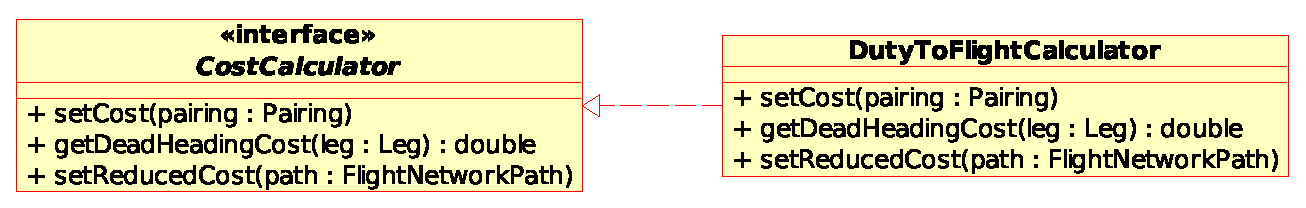
\includegraphics[scale=0.65]{fig/cost_calculator.eps}
		\caption{Interface {\it CostCalculator} e a sua relação com a implementação concreta
    DutyToFlightCalculator. Note que com esse acoplamento diversas implementações para o cálculo do
    custo são possíveis.}
		\label{fig:cost_interface}
	\end{center}
\end{figure}


%%%%%%%%%%%%%%%%%%%%%%%%%%%%%%%%%%%%%%%%%%%%%%%%%%%%%%%%%%%%%%%%%%%%%%%%%%%%%%%%%%%%%%%%%%%%%%%%%%%%

\subsection{Algumas Métricas do Código}
\label{sec:metricas}

Através do {\it plugin} Metrics do Eclipse obtivemos algumas informações sobre o código: 

\begin{itemize}
\item 55\% de cobertura de testes. Os métodos heurísticos são difíceis de se testar e por isso a
cobertura total foi reduzida. No entanto, a base do código teve cerca de 80\% de cobertura e 
garantiu a robustez desejada;
\item 5600 linhas de código; 
\item 3,6 linhas de código por método; 
\item 16 pacotes; 
\item 78 classes; 
\item 795 métodos.
\end{itemize}

%%%%%%%%%%%%%%%%%%%%%%%%%%%%%%%%%%%%%%%%%%%%%%%%%%%%%%%%%%%%%%%%%%%%%%%%%%%%%%%%%%%%%%%%%%%%%%%%%%%%

\zerar
\chapter{Conclusão}
\label{cap:conclusao}

Com relação a análise preliminar apresentada na Seção~\ref{sec:preliminar}, concluímos que o
procedimento de geração de viagens leva a um número gigantesco de variáveis, mesmo para um pequeno
número de pernas (Figura~\ref{fig:pairings}). Isso porque a natureza combinatória do problema leva o
algoritmo de busca a explorar diversas possibilidades, principalmente em uma rede como a da ponte
aérea, onde existem diversas possibilidades de conexão toda vez que se chega em uma das localidades.
Além disso, essas possibilidades se multiplicam quando consideramos um maior número de jornadas
permitidas (\verb|MAX_DUTIES|). Apesar disso, a geração de viagens ainda se fez em tempo aceitável,
podendo ser aplicada para redes maiores (Figura~\ref{fig:generation}).

Entretanto, quando esse número enorme de variáveis é levado ao otimizador, o tempo de processamento
se torna impraticável. Para se certificar disso, basta extrapolar as curvas obtidas nas
Figuras~\ref{fig:glpk} e~\ref{fig:cplex}. Uma tentativa de resolução de uma instância da ponte-aérea
contendo 40 etapas, não pode ser resolvida mesmo após 12 horas de processamento. Ainda assim,
ficamos surpresos com a capacidade do otimizador resolver instâncias com um número de variáveis da
ordem de $10^6$ em tempo aceitável (resultados da Tabela~\ref{tab:resultados}).

A análise preliminar então nos mostra que o método de ``gerar-e-otimizar'' não é adequado para
resolver o problema de forma geral. Em particular, das milhares de variáveis geradas, apenas poucas
delas são escolhidas para entrar na solução final, como se pode observar da
Tabela~\ref{tab:resultados}. Isso indica que o procedimento de geração explícita de variáveis não é
adequado, pois muitas delas não servem para nada. Um procedimento mais inteligente seria o de gerar
apenas variáveis ``boas'', ou seja, com grande chance de aparecerem na solução final. O método de
geração de colunas é o que desenvolve essa ideia.

Com relação aos resultados exatos obtidos utilizando o modelo {\it set cover} (\ref{eq:scpdv}), 
observamos que como as colunas associadas às variáveis $y_i$ foram ajustadas com preços altos, e 
como os problemas analisados eram viáveis do ponto de vista do {\it set partition}, o otimizador 
encontrou as mesmas soluções que seriam obitidas sem a presença de {\it deadheading}. Assim, a 
presença de {\it deadheading} na solução só existirá se for estritamente necessária para 
viabilidade do problema. Infelizmente apenas os problemas P1, P2 e P3 da Tabela~\ref{tab:problemas}
puderam ser resolvidos exatamente.

Analisando a heurística da busca local, podemos tirar mais algumas conclusões com relação ao
parâmetro $k$ de sua implementação. Em nossos testes, utilizamos três valores distintos para $k$ 
e com base nos dados da Tabela~\ref{tab:comparacao} e gráficos da Figura~\ref{fig:ls_results} 
podemos afirmar:

\begin{itemize}
\item $k = 2$: Pode ser visto facilmente nos gráficos que o algoritmo converge para mínimos locais
rapidamente, apresentando ganhos pequenos por iteração. Além disso, muitas iterações não resultam em
melhoria pois os subproblemas resultantes da escolha de duas viagens são normalmente inviáveis ou já
são ótimas; 
\item $k = 3$: Mostrou-se o valor mais eficiente para k pois apresentou uma boa convergência e
iterações mais rápidas do que $k = 4$. Para obter soluções tão boas quanto $k = 4$, torna-se
necessário um número maior de iterações.
\item $k = 4$: Converge em poucas iterações em direção ao ótimo mas cada iteração necessita de um
tempo maior de processamento.
\end{itemize}

O algoritmo genético híbrido proposto apresenta dependência sensível de desempenho com relação a
seus parâmetros. Em particular, o número de vezes, $L$, que cada indivíduo da população inicial é
iterado pelo método de busca local, foi variado em nossos testes. Para cada valor de $L$ utilizado,
chegamos as seguintes conclusões:

\begin{itemize}
\item $L = 1$: Uma iteração por indivíduo não foi suficiente para gerar melhorias significativas na
convergência;
\item $L = 5$: Tornou mais rápida a convergência, mostrando a utilização de busca local tem um
impacto positivo nos resultados;
\item $L = 10$: Para instâncias pequenas teve influência similar ao $L = 5$, no entanto para a
instância 73G\_340, seu desempenho foi muito superior. Isso indica que quanto maior o número de
voos, maior é o valor de $L$ que maximiza os ganhos de performance.
\end{itemize}

O método de geração de coluna implementado se mostrou bastante eficiente para a resolução da
relaxação linear associada ao problema. Entretanto, para as instâncias grandes, os subconjuntos de
viagens geradas não foram pequenos o suficiente para que pudéssemos resolver o problema linear
inteiro com essas variáveis. Ou seja, não foi possível obter uma solução inteira utilizando as
colunas geradas.

Heurísticas ainda podem ser aplicadas no sentido de se diminuir o subconjunto de viagens geradas,
possibilitando a resolução do problema inteiro. Por exemplo, podemos restringir o número máximo de
caminhos encontrados até cada nó do grafo durante a resolução do {\it pricing problem}. Podemos
ainda considerar no final apenas as colunas com custo reduzido abaixo de um valor limite ({\it
cutoff}). Não fizemos a implementação dessas heurísticas nesse trabalho.

Para resumir, listamos a seguir em forma de tópicos algumas conclusões gerais com relação ao
problema estudado neste projeto:

\begin{itemize}
\item O problema de geração de viagens é muito mais complexo do que aparenta. 
\item O problema realmente necessita de métodos aproximados devido à incapacidade dos métodos exatos
em resolver instancias grandes.
\item Uma solução otimizada realmente pode gerar uma grande economia à empresa aérea.
\item Ainda há muito espaço para pesquisas nessa área. 
\item O problema de otimização de viagens é apenas parte de um problema maior que seria o
escalonamento dos tripulantes.
\end{itemize}

%%%%%%%%%%%%%%%%%%%%%%%%%%%%%%%%%%%%%%%%%%%%%%%%%%%%%%%%%%%%%%%%%%%%%%%%%%%%%%%%%%%%%%%%%%%%%%%%%%%%

\section{Perspectivas Futuras}
\label{sec:perspectivas}

O desenvolvimento do projeto mostrou-se satisfatório. Entretanto sentimos que ainda há espaço para
efetuarmos algumas melhorias e novas implementações. Por exemplo, não foi possível ainda obter uma
solução inteira a partir do preocedimento de geração de colunas. A técnica utilizada para isso é
conhecida por {\it branch-and-price}~\cite{vance97h} e consiste basicamente em aplicar o
procedimento de geração de colunas em cada nó da árvore enumerativa da técnica {\it
branch-and-bound} usual. Acreditamos que o trabalho desenvolvido até então fornece uma boa base para
implementar essa técnica.

Outro ponto interessante do trabalho foi analisar os pontos fortes de cada heurística estudada. A
partir desse conhecimento, acreditamos que seja possível combinar as três heurísticas em um novo
algoritmo híbrido. A ideia inicial seria utilizar as colunas produzidas pelo método geração de
colunas como entrada para o algoritmo genético híbrido a fim de se obter uma solução inteira
aproximada. Essa, por sua vez, poderia ser refinada através do procedimento de busca local.
Novamente, acreditamos que a implementação dessa nova heurística possa ser realizada de forma
simples, dada a base desenvolvida durante esse trabalho.

Uma outra possibilidade de exploração futura seria a paralelização de partes importantes do código,
visando um melhor desempenho no contexto da computação paralela e distribuída. Por exemplo, o
procedimento de geração de viagens pode ser facilmente paralelizavel.

Resumidamente, os pontos que podem ser explorados futuramente são listados abaixo:

\begin{itemize} 
\item Implementação de um esquema {\it branch-and-price} para obtenção de solução inteira a partir
da geração de colunas;
\item Combinação e paralelização das heurísticas estudadas, explorando os pontos fortes de cada uma
delas;
\item Possível sistema comercial.
\end{itemize}

%%%%%%%%%%%%%%%%%%%%%%%%%%%%%%%%%%%%%%%%%%%%%%%%%%%%%%%%%%%%%%%%%%%%%%%%%%%%%%%%%%%%%%%%%%%%%%%%%%%%

\bibliography{../bib/crew_scheduling}
\bibliographystyle{plain}

\part{Conteúdo Subjetivo}

\chapter{Sobre o BCC}
\label{cap:bcc}


%\newpage
\section{Lucas Rodrigues Colucci}
\label{sec:lucas_subjetiva}

%\section{Renato Lerac Corrêa de Sá}
\label{sec:renato_subjetiva}

\end{document}

